\chapter{Finite Element Modeling}
\label{chap:FEM}

This chapter outlines the development of the finite element model of the X-Wagen metro and the simulation setup. First, in section \ref{section:geometry}, the design of the model geometry and the mesh of the computational model are shown. Consecutively, section \ref{section:boundary_conditions} describes the incorporation of boundary conditions into the finite element model and the modeling approach of the loudspeaker sound source. Finally, in section \ref{section:parametric_study}, a parametric study is carried out to investigate the influence of different simulation parameters on the solution of the initial finite element model. All these simulations are executed with the acoustics module of the open-source FEM software openCFS \cite{opencfs}.


\section{Geometry and mesh}
\label{section:geometry}

Due to the large dimension of the vehicle (about \SI{19}{\meter} long per metro car), a simulation on the complete metro train would be too extensive from the computational point of view. Hence, the modeling domain has to be confined to a selected section of the car, which constitutes of the front non-driven bogie at the head car of the metro only. The latter has been marked through a red box in \cref{fig:red_box}. Furthermore, the outer pressure field measurement described in \cref{sec:pressure_field_measurement} has been taken from the same area.

\begin{figure}
	\centering
	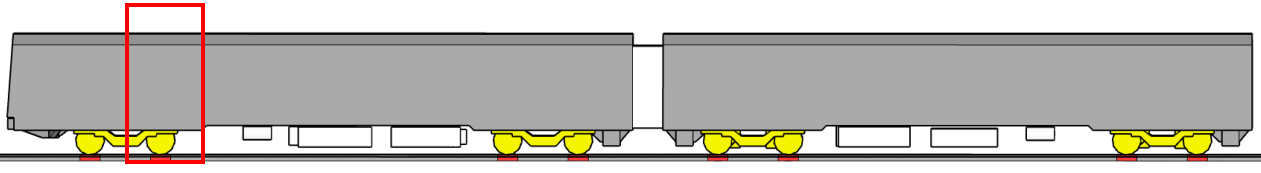
\includegraphics[width=\textwidth]{fig/chap4/geometry/model_area.png}
	\caption{Side view of the X-Wagen 3D model, red box indicates the modeling area.}
	\label{fig:red_box}
\end{figure}

The geometry of the modeled car section consists of the car body shell and the non-driven bogie. The dimension parameters of the modeled components are measured from the 3D model of the X-Wagen (see \cref{fig:ubx_sketup_model} and \cref{fig:bogie_model}). It has been shown in \cref{section:ubx_geometry}, if the brake disc and the brake caliper are disregarded, the symmetry of the bogie can be exploited. Furthermore, due to the symmetry of the car body shell in its width and length direction, only one-fourth of the car section is modeled in order to reduce computational effort. The quarter model of the car section is depicted in \Cref{fig:fourth_model}, whereas the equivalent model, namely the full model, is shown in \cref{fig:full_model}. Both models are shown for more comprehensive illustration of the model geometry, but only the quarter model has been used in the simulation. For simplification of the geometry design, exclusively the most essential components have been included in the model. As shown in \Cref{fig:fourth_model}, the contemplated components are the squared car body shell (dark green), the bogie frame (purple), the wheel with axle (pink) and the air suspension (gray). The omnidirectional loudspeaker (bright green) is represented through a sphere with \SI{35}{\centi\meter} and is placed at the exact same position as in the validation measurement (see \cref{fig:loudspeakerposition}). 

\begin{figure}
	\centering
	\begin{subfigure}[b]{0.4\textwidth}
		\centering
		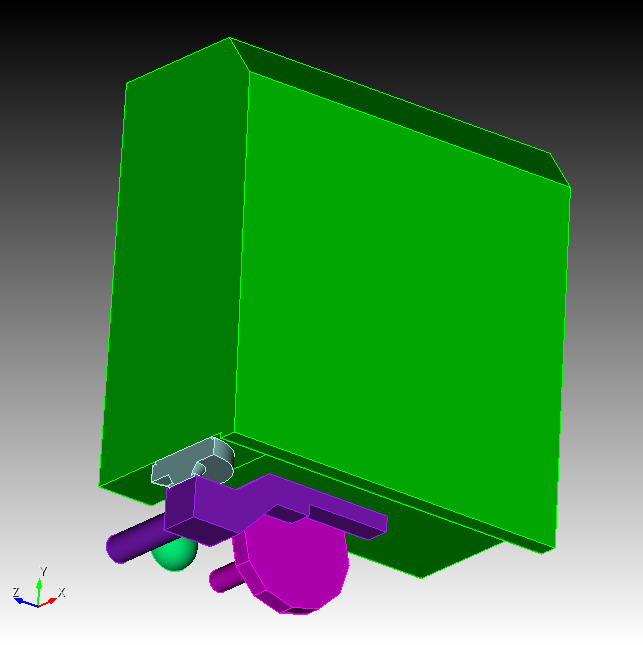
\includegraphics[width=0.9\linewidth]{fig/chap4/geometry/one_fourth_model.png}
		\caption{One-fourth model.}
		\label{fig:fourth_model}
	\end{subfigure}
	\hfill
	\begin{subfigure}[b]{0.4\textwidth}
		\centering
		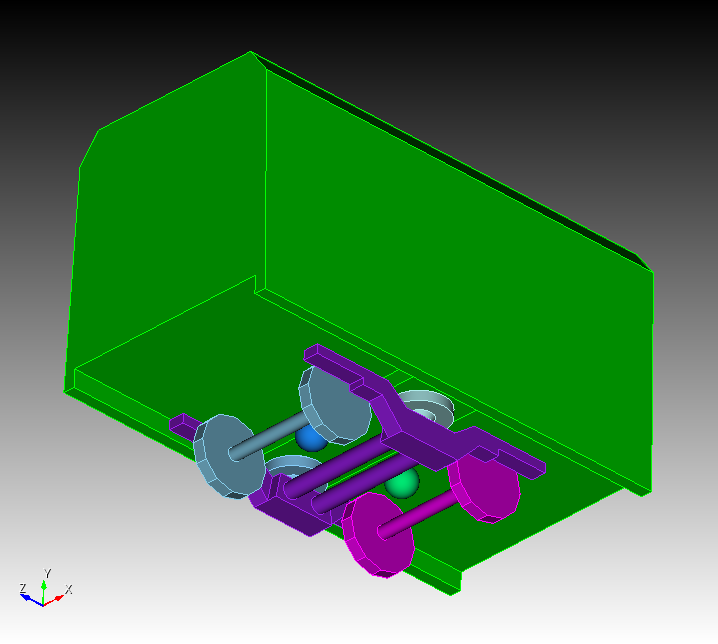
\includegraphics[width=\linewidth]{fig/chap4/geometry/initial_model_2.png}
		\caption{Full model.}
		\label{fig:full_model}
	\end{subfigure}
	\caption{Geometry of the modeled car section. The full model is shown for better illustration. The one-fourth model has been used for the simulation.}
\end{figure}

After the car section geometry is designed, the actual computational model (see \cref{fig:regions}) used for the acoustic simulation is obtained by cutting the car section model out of a acoustic fluid (in this case, air) volume. Likewise, only one fourth of the volume is considered due to the symmetry of the problem. Since the radiation of the underfloor noise into the free field around the vehicle is of interest, the acoustic region is surrounded by a perfectly matched layer ($\Omega_{\text{PML}}$) to model the open domain. To reduce the effort of the latter meshing process of the model geometry, the propagation region is divided into two subregions, namely the region that contains the cut out bogie components ($\Omega_1$) and the main propagation region ($\Omega_2$), respectively. The main propagation region has the same length as the one-fourth car section model of \SI{2.6}{\meter} and a height of \SI{4.52}{\meter} so that the upper boundary of the acoustic region is about \SI{1}{\meter} above the car roof. The choice of the propagation domain width needs to be well-considered. While using a insufficient domain width i.e. with the PML being placed very close to the acoustic source would cause nonphysical reflection of the acoustic wave at the regions interface, setting the domain width too large would increase the computational effort of the simulation extensively. According to several PML usage guidelines \cite{PML_comsol, PML_quickwave, PML_3ds}, a minimum distance of half of the simulation frequency wavelength ($\lambda/2$) to the radiating source is recommended. This criteria is fulfilled for the domain height (\SI{4.52}{\meter}) and the length (\SI{2.6}{\meter}) using the lowest simulation frequency of \SI{100}{\hertz} ($\lambda / 2 = 1.71\,\text{m}$). The actual domain width used for the simulation will be determined in a latter parameter study.

\begin{figure}
	\centering
	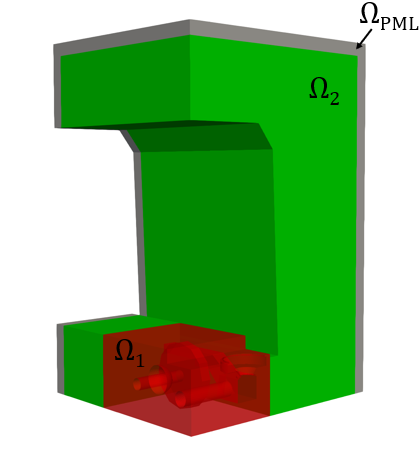
\includegraphics{fig/chap4/mesh/region_small.png}
	\caption{Computational model consists of a acoustic fluid (air) volume surrounded by a PML domain ($\Omega_{\text{PML}}$). The acoustic domain is divided into two subregions $\Omega_1$ and $\Omega_2$ for a easier meshing of the geometry. Thereby, $\Omega_1$ is displayed semi-transparently to illustrate the outlines of the cut out bogie components.}
	\label{fig:regions}
\end{figure}
% mesh element type
Subsequently, a mesh of the model geometry (see \cref{fig:mesh}) was created using Coreform Cubit \cite{cubit} mesh generator, which offers several advanced semi-automatic meshing techniques that can extensively lower the effort of the meshing process. The subregion $\Omega_1$ contains complex outlines of the bogie components, and is therefore meshed using tetrahedral elements, which are perfectly suitable for meshing complex geometries but are more computationally expensive than the hexahedral elements. To lower the computational cost of the model, the main propagation region $\Omega_2$ is meshed using hexahedral elements. For both regions, second-order (quadratic) element type is used (p-refinement) to reduce discretization errors, which is computationally more efficient than using a smaller element size (h-refinement) \cite{Kuo_2007_prefinement}.
% non-conforming interface
Special care needs to be taken if a hex-tet mesh combination is used. Thereby, the subregions $\Omega_1$ and $\Omega_2$ are coupled by non-conforming interfaces $\Gamma_\text{NC}$, which allow different element types to be used in the same mesh. For the simulation, the default setup of the non-conforming interface in openCFS is used, which if of type Nitsche. For detailed information of non-conforming interfaces, one can refer to e.g. Roppert et al. 2020 \cite{Roppert_2020_nc_interface}.
% PML region
For the PML region $\Omega_{\text{PML}}$, Kaltenbacher \cite{KALTENBACHER_PML_2013} recommended using a least four linear elements and two quadratic elements in the PML thickness direction and using the same spatial discretization as of the acoustic domain. For the sake of enhancing the stability of the performance of the PML, three quadratic hexahedral elements are used in the mesh of the finite element model. The damping function used in the PML region is the inverse distance damping (see \cref{eq:inverse_dis}), which is default in openCFS.
% mesh size
Through a preliminary study of the problem, the frequency analysis range of the simulation is set to \SIrange{100}{2000}{\hertz} in one-third octave bands, resulting 14 frequency bands in the given range, which are shown in \cref{tab:third_octave_bands_used}. As can be read from the table, the lower and the upper limit of the frequency analysis are 89 Hz and 2262 Hz, respectively. Due to the broad range of the analyzed frequencies, using a constant mesh size covering the entire range would be challenging. On the one hand, using a mesh size corresponding to the highest simulation frequency for all frequencies would be computational too expensive, on the other hand, using a mesh size that is designed for lower frequency bands would increase discretization errors in higher frequency bands, since the wavelength would be resolved insufficiently. The solution of this problem is to choose a mesh discretization depending on the analysis frequency band. For the finite element simulation of the X-Wagen, four different grids as shown in \cref{tab:grid_size} are prepared. The discretization size is chosen so that the wavelength corresponding to the upper cutoff frequency of the analyzed one-third octave band is resolved by at least 6 elements i.e. $h = \lambda_{f_u} / 6$, which also means for any frequencies lower, the discretization is getting finer. The bogie components contain complex and more importantly small surfaces that require a fine discretization size of the surface mesh, which is not fulfilled for low frequency band like 100 Hz ($\lambda_{\text{\SI{100}{\hertz}}} / 6 = 0.57\,\text{m}$). It has been shown hat using a discretization size corresponding to the wavelength of 1000 Hz (h = \SI{0.057}{\meter}) could mesh the surfaces adequately. Hence, this grid size is used for the one-third octave bands from \SIrange{100}{800}{\hertz}. Since the upper frequency limit of the \SI{1000}{\hertz} band is greater than \SI{1000}{\hertz}, a finer grid size would be necessary so that the mentioned discretization criteria still holds. Hence, the \SI{1000}{\hertz} band and the \SI{1250}{\hertz} band share the same grid size of \SI{0.036}{\meter}. For the highest frequency bands \SI{1600}{\hertz} and \SI{2000}{\hertz}, individual grid sizes are used, respectively.
The above mentioned parameters of the mesh of the finite element model as well as the material parameters used for the acoustic domain are summarized in \cref{tab:model_parameters}.

\begin{figure}
	\centering
	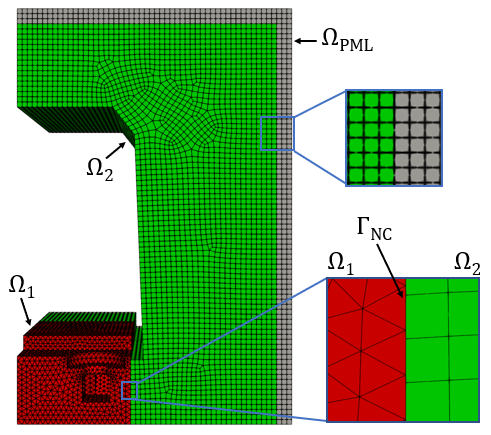
\includegraphics{fig/chap4/mesh/Mesh_with_labels_small.png}
	\caption{Mesh of the computational model. The acoustic subregions $\Omega_1$ and $\Omega_2$ are meshed with tetrahedral and hexahedral elements, respectively. Both subregions are coupled with non-conforming interfaces $\Gamma_\text{NC}$ of Nitsche type. For the PML region $\Omega_{\text{PML}}$, a constant number of three quadratic hexahedral elements along the thickness direction are used. All regions $\Omega_1$, $\Omega_2$, $\Omega_{\text{PML}}$ share the same maximum element size, which is frequency-dependent as shown in \cref{tab:grid_size}.}
	\label{fig:mesh}
\end{figure}

\begin{table}
	\centering
	\caption{Parameters of the computational model.}
	\label{tab:model_parameters}
	\begin{tabular}{lc}
		\toprule
		Parameter & Value \\
		\midrule
		\textbf{Propagation region} & \\
		Element type $\Omega_1$ & quadratic tetrahedral element \\
		Element type $\Omega_2$ & quadratic hexahedral element \\
		Maximum element size $\Omega_1$, $\Omega_2$ & frequency-dependent, see \cref{tab:grid_size}\\
		\textbf{PML region} & \\
		Number of PML elements along thickness direction & 3 \\
		PML element type & quadratic hexhedral element \\
		PML element size & same as $\Omega_1$, $\Omega_2$\\
		Damping function type & inverse distance damping, see \cref{eq:inverse_dis} \\
		\textbf{Non-conforming interface} & \\
		Master domain & $\Omega_1$ \\
		Slave domain & $\Omega_2$ \\
		Type of mortaring & Nitsche (OpenCFS defalut) \\
		Penalization-parameter & 100 (OpenCFS default) \\
		\textbf{Material (air at \SI{20}{\degreeCelsius})} & \\
		Density $\rho_0$ & \SI{1.204}{\kilogram\per\cubic\meter} \\
		Bulk modulus $K$ & \SI{142}{\kilo\pascal} \\
		Speed of sound $c_0$ & \SI{343.21}{\meter\per\second} \\
		Characteristic acoustic impedance $Z_0$ & \SI{413.3}{\pascal\second\per\meter}  \\
		\bottomrule
	\end{tabular}
\end{table}

\begin{table}
	\centering
	\caption{One-third octave bands used for the simulation. The quantities $f_{\text{c}}$, $f_{\text{l}}$, $f_{\text{u}}$ denote the center frequency, the lower cutoff frequency and the upper cutoff frequency of the corresponding frequency band, respectively.}
	\label{tab:third_octave_bands_used}
	\begin{tabular}{cccccc}
		\toprule
		Band & $f_{\text{c}}$ (Hz) & $f_{\text{l}}$ - $f_{\text{u}}$ (Hz) & Band & $f_{\text{c}}$ (Hz) & $f_{\text{l}}$ - $f_{\text{u}}$ (Hz) \\
		\midrule
		1 & 100 & 89 - 112 & 8 & 500 & 449 - 565 \\
		2 & 125 & 112 - 141 & 9 & 630 & 565 - 713 \\
		3 & 160 & 141 - 178 & 10 & 800 & 713 - 897 \\
		4 & 200 & 178 - 224 & 11 & 1000 & 897 - 1131 \\
		5 & 250 & 224 - 283 & 12 & 1250 & 1131 - 1425 \\
		6 & 315 & 283 - 356 & 13 & 1600 & 1425 - 1796 \\
		7 & 400 & 356 - 449 & 14 & 2000 & 1796 - 2262 \\
		\bottomrule
	\end{tabular}
\end{table}


\begin{table}
	\centering
	\caption{Frequency-dependent discretization size of computational grids.}
	\label{tab:grid_size}
	\begin{tabular}{ccc}
		\toprule
			& Used for one-third octave bands (Hz) & Discretization size h (m) \\
		\midrule
		Grid 1 & 100, 125, 160, 200, 250, 315, 400, 500, 630, 800 & 0.057 \\
		Grid 2 & 1000, 1250 & 0.036 \\
		Grid 3 & 1600 & 0.029 \\
		Grid 4 & 2000 & 0.025 \\
		\bottomrule
	\end{tabular}
\end{table}


\subsection*{Variation of the simulation domain width}

The aim of this parameter study is to find an appropriate simulation domain size that provides sufficient numerical accuracy while keeping the computational effort of the simulation in a adequate range. Thereby, the length and the height of the main propagation region $\Omega_2$ are kept constant while varying only the width of the domain. In what follows, the domain width is defined as the distance between the lower edge of the car body wall and the outer boundary of the main propagation region $\Omega_2$, as depicted in \cref{fig:domain_width_2m}. For the parameter study, 5 different domain widths are used, which are \SI{0.2}{\meter}, \SI{0.5}{\meter}, \SI{1}{\meter}, \SI{1.5}{\meter} and \SI{2}{\meter}, respectively. The model with the smallest and the largest width are shown in \cref{fig:domain_size_variation}, respectively. According to several PML usage guidelines \cite{PML_3ds, PML_comsol, PML_quickwave}, placing the PML at a distance of half of the wavelength to the radiating source would be sufficient for most of the cases. For our simulation, it would be \SI{1.71}{\meter}, which is the half of the wavelength corresponding to the lowest analysis frequency \SI{100}{\hertz}. Hence, the reference solution is computed by using the model with \SI{2}{\meter} width and all errors are evaluated with respect to this reference. For the simulation, a fictitious excitation with uniform normal surface particle velocity of $u_s$ = \SI{1}{\milli\meter\per\second} is applied to the loudspeaker surface. And the acoustic pressure is evaluated at \SI{0.1}{\meter} away from the vehicle along the height direction as indicated by the vertical red lines in \cref{fig:domain_width_0pt2m} and \cref{fig:domain_width_2m}. Along the height direction, the evaluation points of the acoustic pressure are \SI{0.05}{\meter} from each other, starting from \SI{0}{\meter} and ending with \SI{4.5}{\meter}, resulting 91 evaluation positions in total. At each evaluation point, the relative error of the acoustic pressure value $\hat{p}_{a,i}$ (real part and imaginary part) to the reference solution $\hat{p}_{a,\text{ref},i}$ is computed by
\begin{equation}
	E_{p_a,i} = \left(\frac{\left| \hat{p}_{a,i} - \hat{p}_{a,\text{ref},i} \right|}{\left|\hat{p}_{a,\text{ref},i}\right|}\right)100\,\% \,,
\end{equation}
with $i$ being the evaluation position and $i \in \left[1\dots91\right]$. The simulation is carried out with the one-third octave center frequencies from \SIrange{100}{2000}{\hertz}, using the computational grids as displayed in \cref{tab:grid_size}.

The relative error $E_{p_a,i}$ along the domain height direction using different domain widths for frequency \SI{100}{\hertz} and \SI{2000}{\hertz} are shown in \cref{fig:relative_error_over_height}. As can be seen for both frequencies, the smallest domain width has the largest error among all domain widths, and the magnitude of the relative error decreases with increasing domain width. For the same domain width, the relative error depends on the evaluation points and increases with the height, which is due to a decreasing width to height ratio. It can be seen that although the smallest domain width \SI{0.2}{\meter} has a quite large relative error in the higher area (up from \SI{2}{\meter}), for the area below \SI{1}{\meter}, it has a similar level of error as the larger domain. Which means, if only the acoustic pressure at the lower area, for example in the underfloor area of the metro, is of interest, the domain boundary can be set very close to the car body, reducing the computational effort extensively. Same behavior of the relative error has also been shown for other frequencies.

To find a suitable domain width for our finite element model, the maximum relative error $E_{p_a,\text{max}}$ and the average relative error $E_{p_a,\text{max}}$ over all 91 evaluation positions are computed for each one-third octave center frequency. The obtained results are shown in \cref{fig:relative_error_spectrum}, additionally, the concrete values are summarized in \cref{tab:computed_errors}. As can be seen from the results, both maximum error and average error decrease with increasing domain width. Up from the domain width of \SI{1}{\meter}, the maximum relative error among all frequencies is limited by \SI{10}{\percent}, and in terms of the average error, the error is limited by \SI{1.5}{\percent}. Setting a average error limit to \SI{2}{\percent}, which corresponds to a deviation of \SI{0.17}{\decibel} in the sound pressure level, choosing \SI{1}{\meter} to be the domain width of our finite element model would be adequately when considering the rising computational effort using a larger domain width. It has been shown by the simulation that the computational effort using the coarsest grid (Grid 1) with \SI{1.5}{\meter} domain width is still in a good range. Hence, for the computational grid for lower frequency bands (\SIrange{100}{800}{\hertz}) a domain width of \SI{1.5}{\meter} is used to further increase the numerical accuracy of the model.

\begin{figure}
	\centering
	\begin{subfigure}[b]{0.45\textwidth}
		\centering
		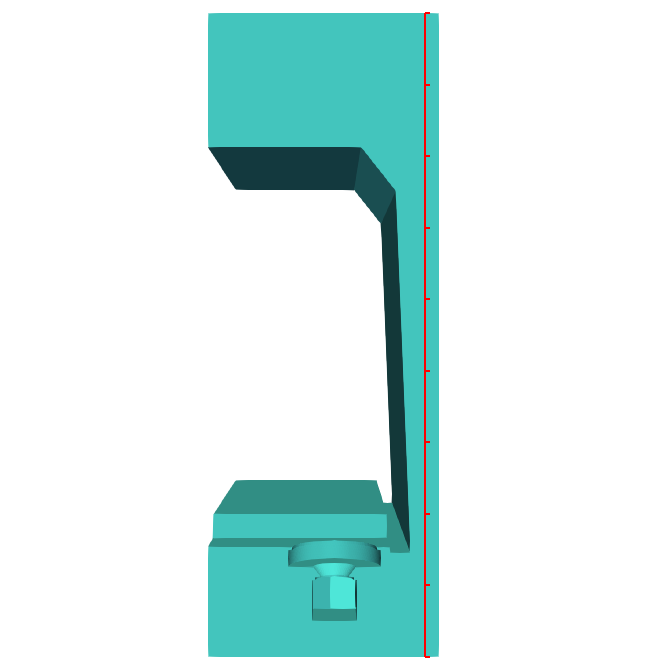
\includegraphics[width=\linewidth]{fig/chap4/simulation_domain/0pt2m.png}
		\caption{0.2 m}
		\label{fig:domain_width_0pt2m}
	\end{subfigure}
	\hfill
	\begin{subfigure}[b]{0.45\textwidth}
		\centering
		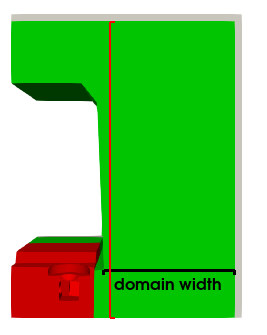
\includegraphics[width=\linewidth]{fig/chap4/simulation_domain/2m.png}
		\caption{2 m}
		\label{fig:domain_width_2m}
	\end{subfigure}
	\caption{Computational models with different propagation domain widths, which are defined as the distance between lower edge of the car body wall and the region outer boundary. The vertical red lines indicate the evaluation position of the acoustic pressure, which is at \SI{10}{\centi\meter} away from the lower car body edge.}
	\label{fig:domain_size_variation}
\end{figure}

\begin{figure}
	\centering
	\begin{subfigure}[b]{0.48\textwidth}
		\centering
		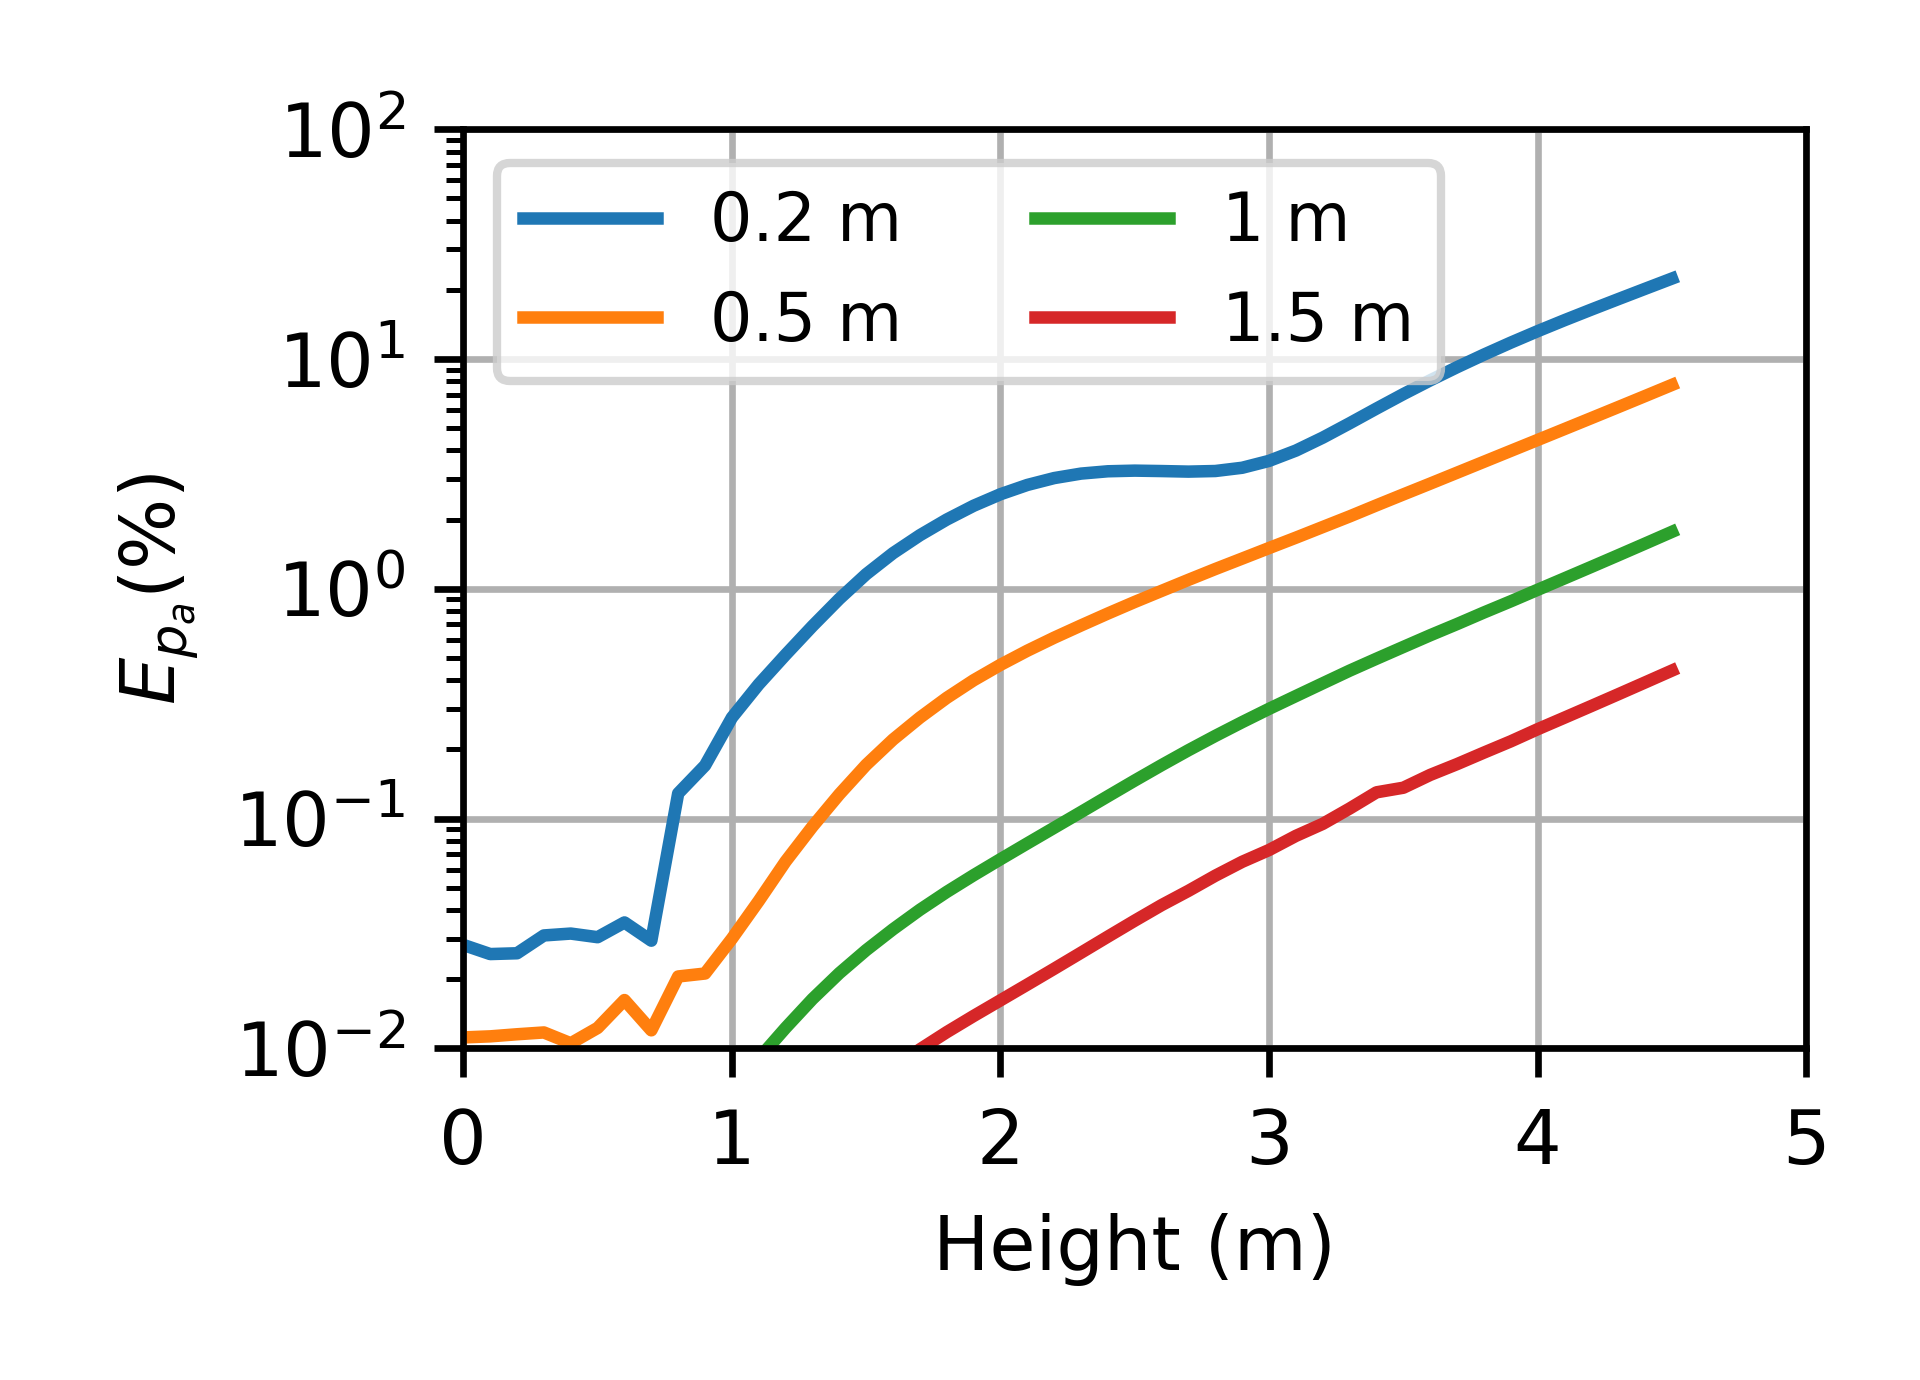
\includegraphics{fig/chap4/simulation_domain/error_100_Hz.png}
		\caption{\SI{100}{\hertz}}
		\label{fig:relative_error_over_height_100Hz}
	\end{subfigure}
	\hfill
	\begin{subfigure}[b]{0.48\textwidth}
		\centering
		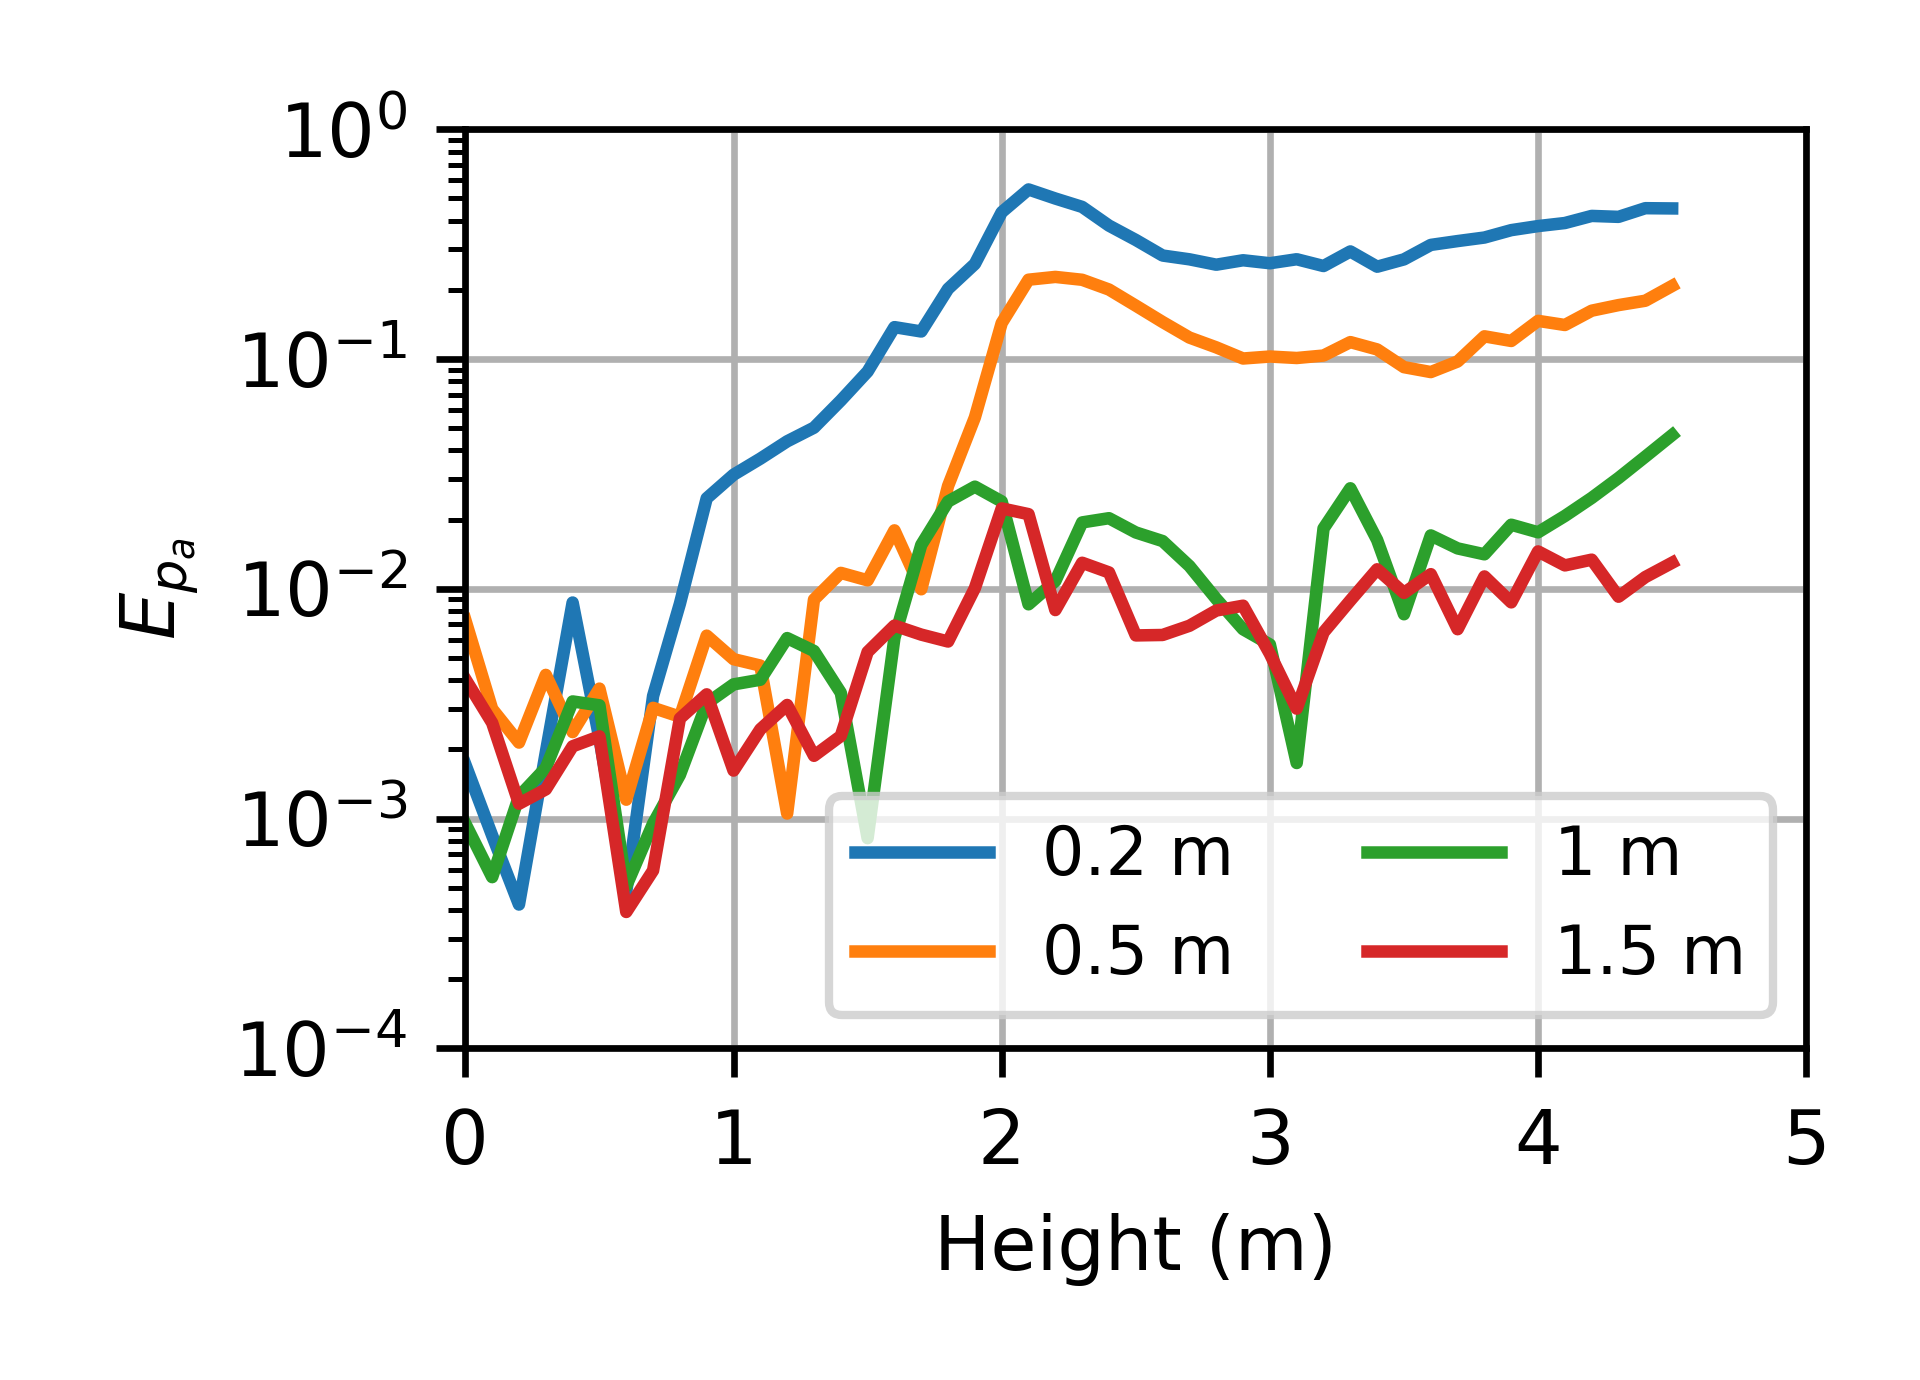
\includegraphics{fig/chap4/simulation_domain/error_2000_Hz.png}
		\caption{\SI{2000}{\hertz}}
		\label{fig:relative_error_over_height_2000Hz}
	\end{subfigure}
	\caption{Relative error $E_{p_a}$ over the domain height for frequency \SI{100}{\hertz} and \SI{2000}{\hertz}.}
	\label{fig:relative_error_over_height}
\end{figure}

\begin{figure}
	\centering
	\begin{subfigure}[b]{0.48\textwidth}
		\centering
		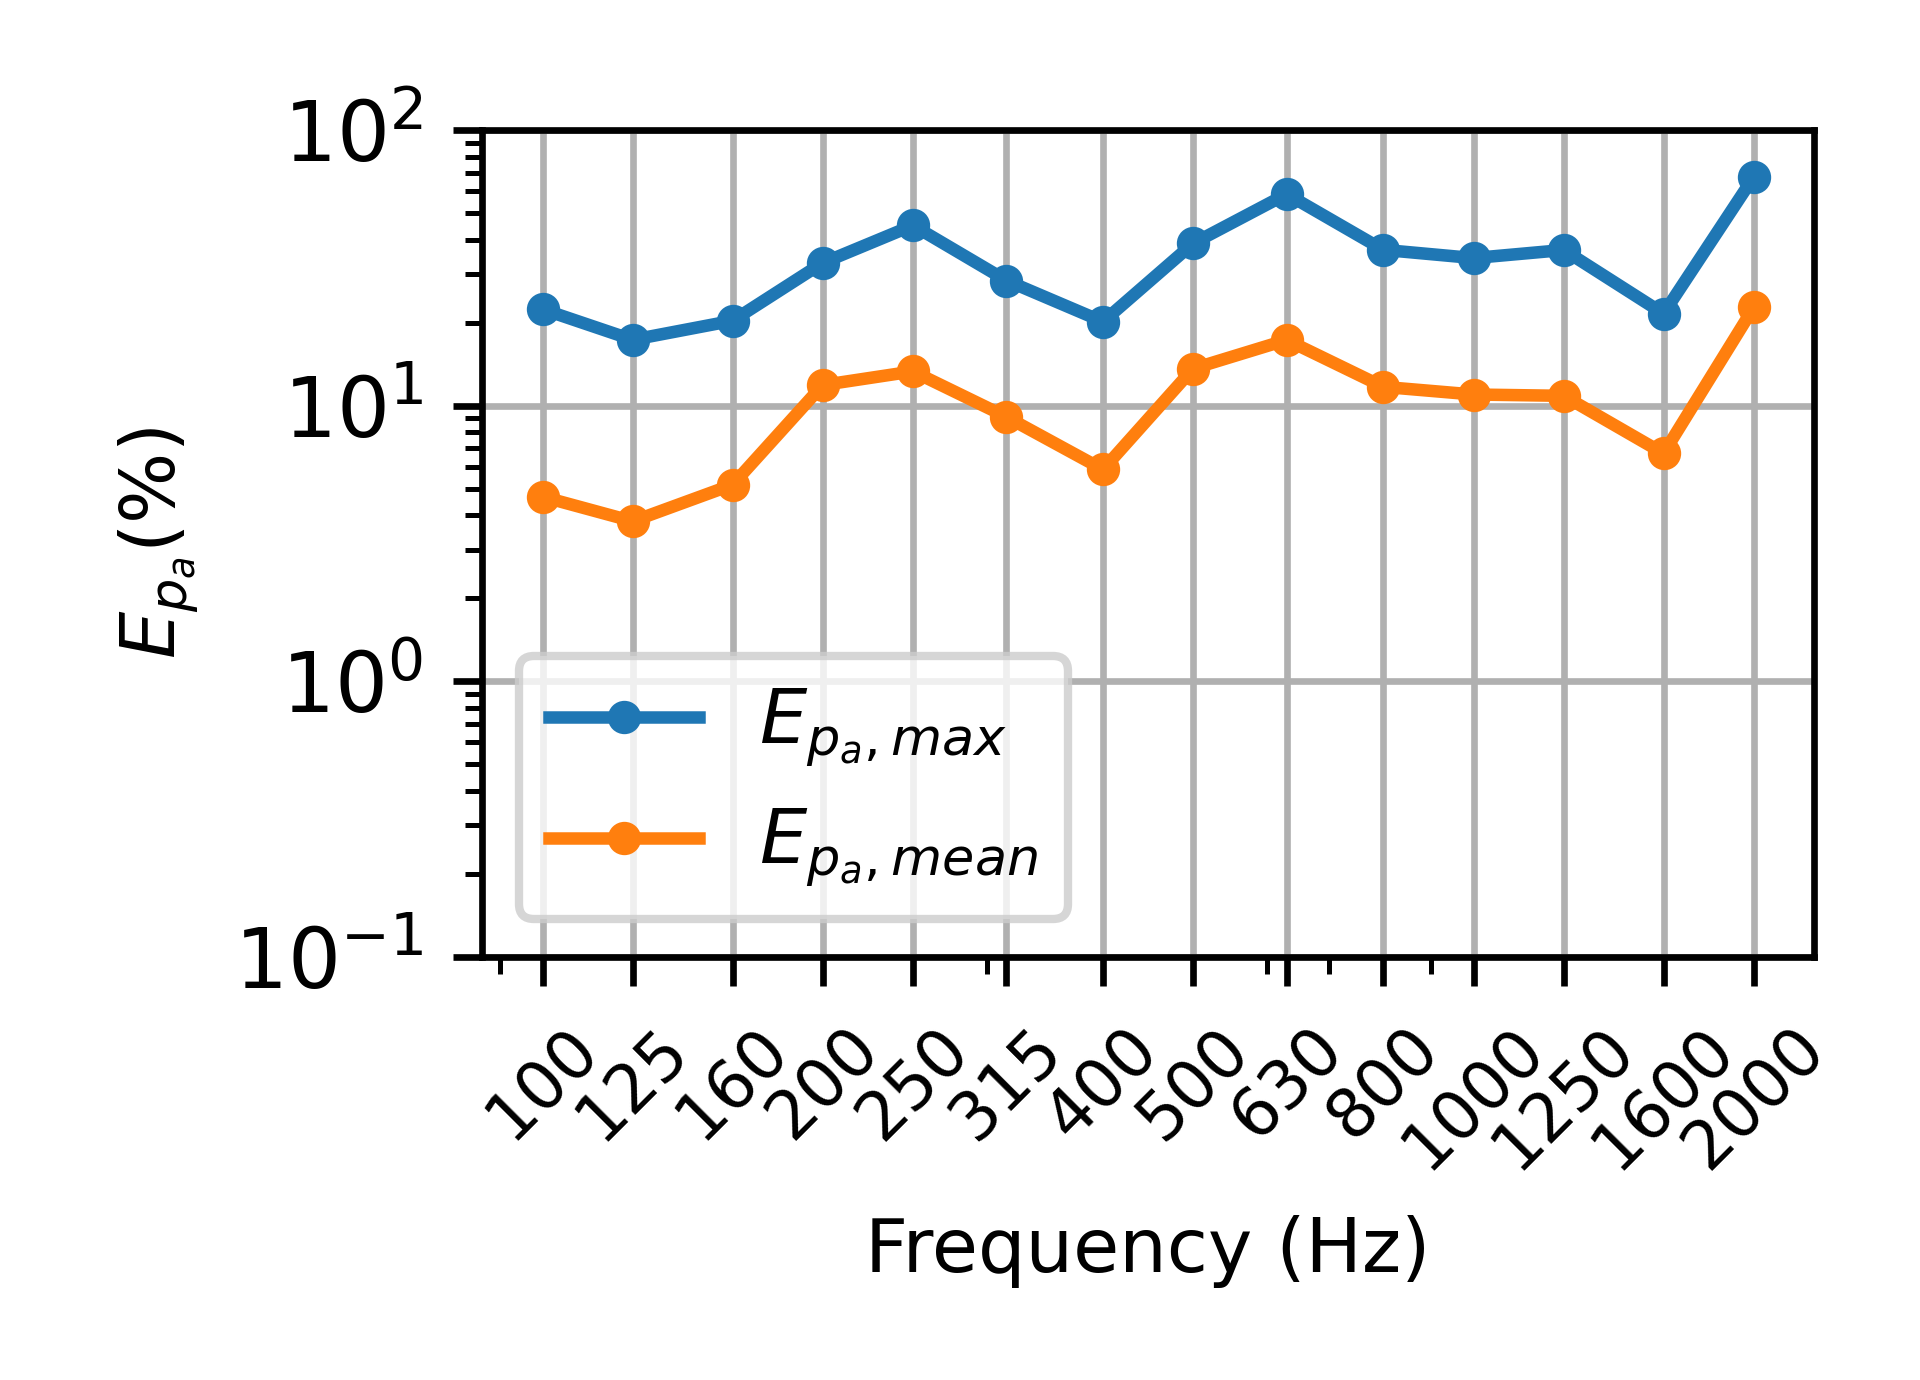
\includegraphics{fig/chap4/simulation_domain/width_0pt2m.png}
		\caption{\SI{0.2}{\meter}}
	\end{subfigure}
	\hfill
	\begin{subfigure}[b]{0.48\textwidth}
		\centering
		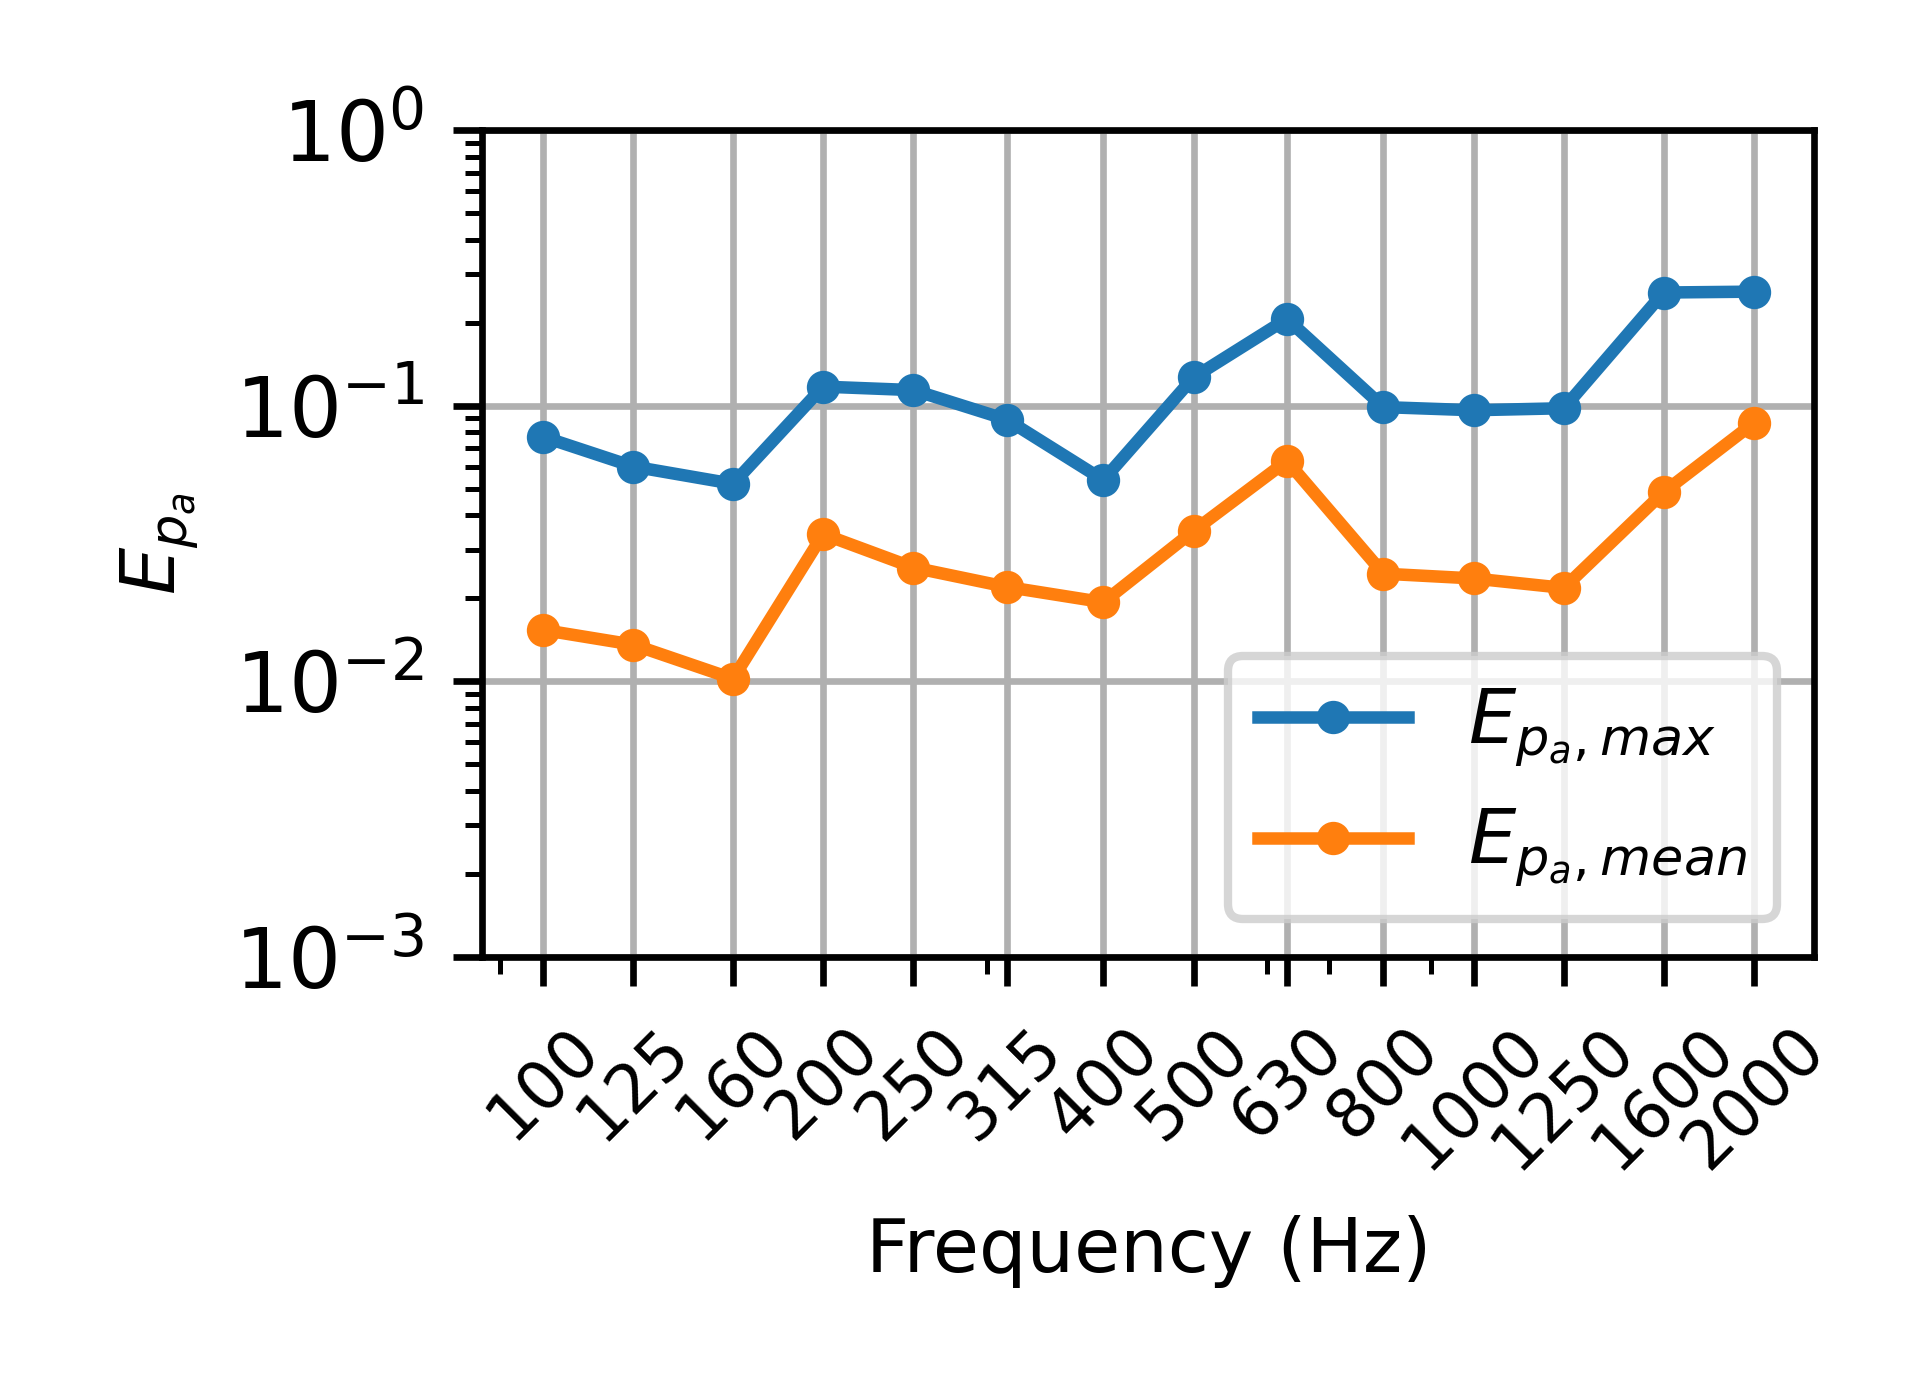
\includegraphics{fig/chap4/simulation_domain/width_0pt5m.png}
		\caption{\SI{0.5}{\meter}}
	\end{subfigure}
	
	\begin{subfigure}[b]{0.48\textwidth}
		\centering
		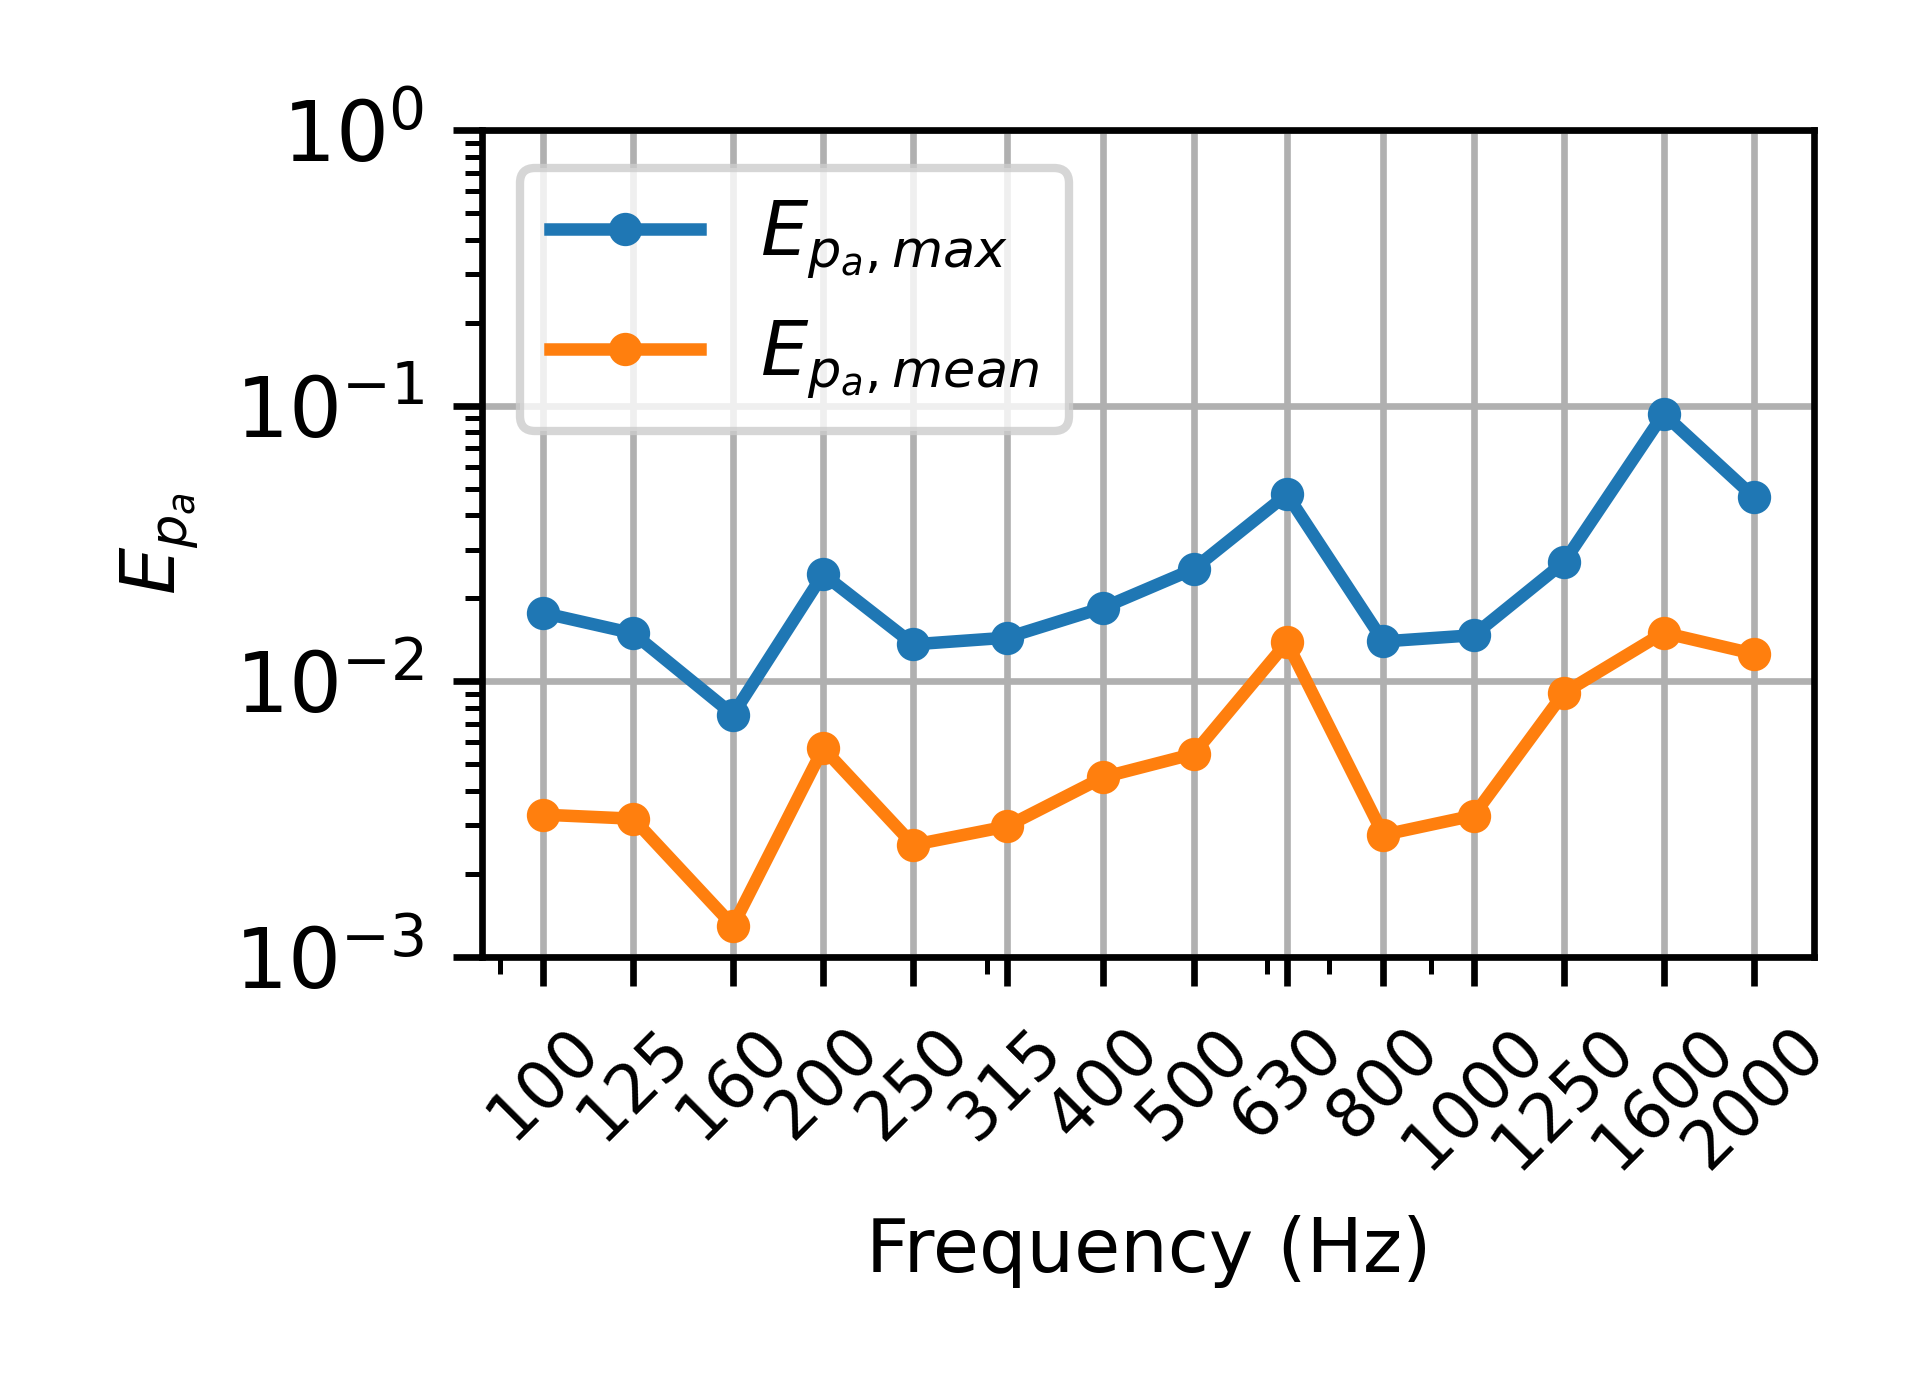
\includegraphics{fig/chap4/simulation_domain/width_1m.png}
		\caption{\SI{1}{\meter}}
	\end{subfigure}
	\hfill
	\begin{subfigure}[b]{0.48\textwidth}
		\centering
		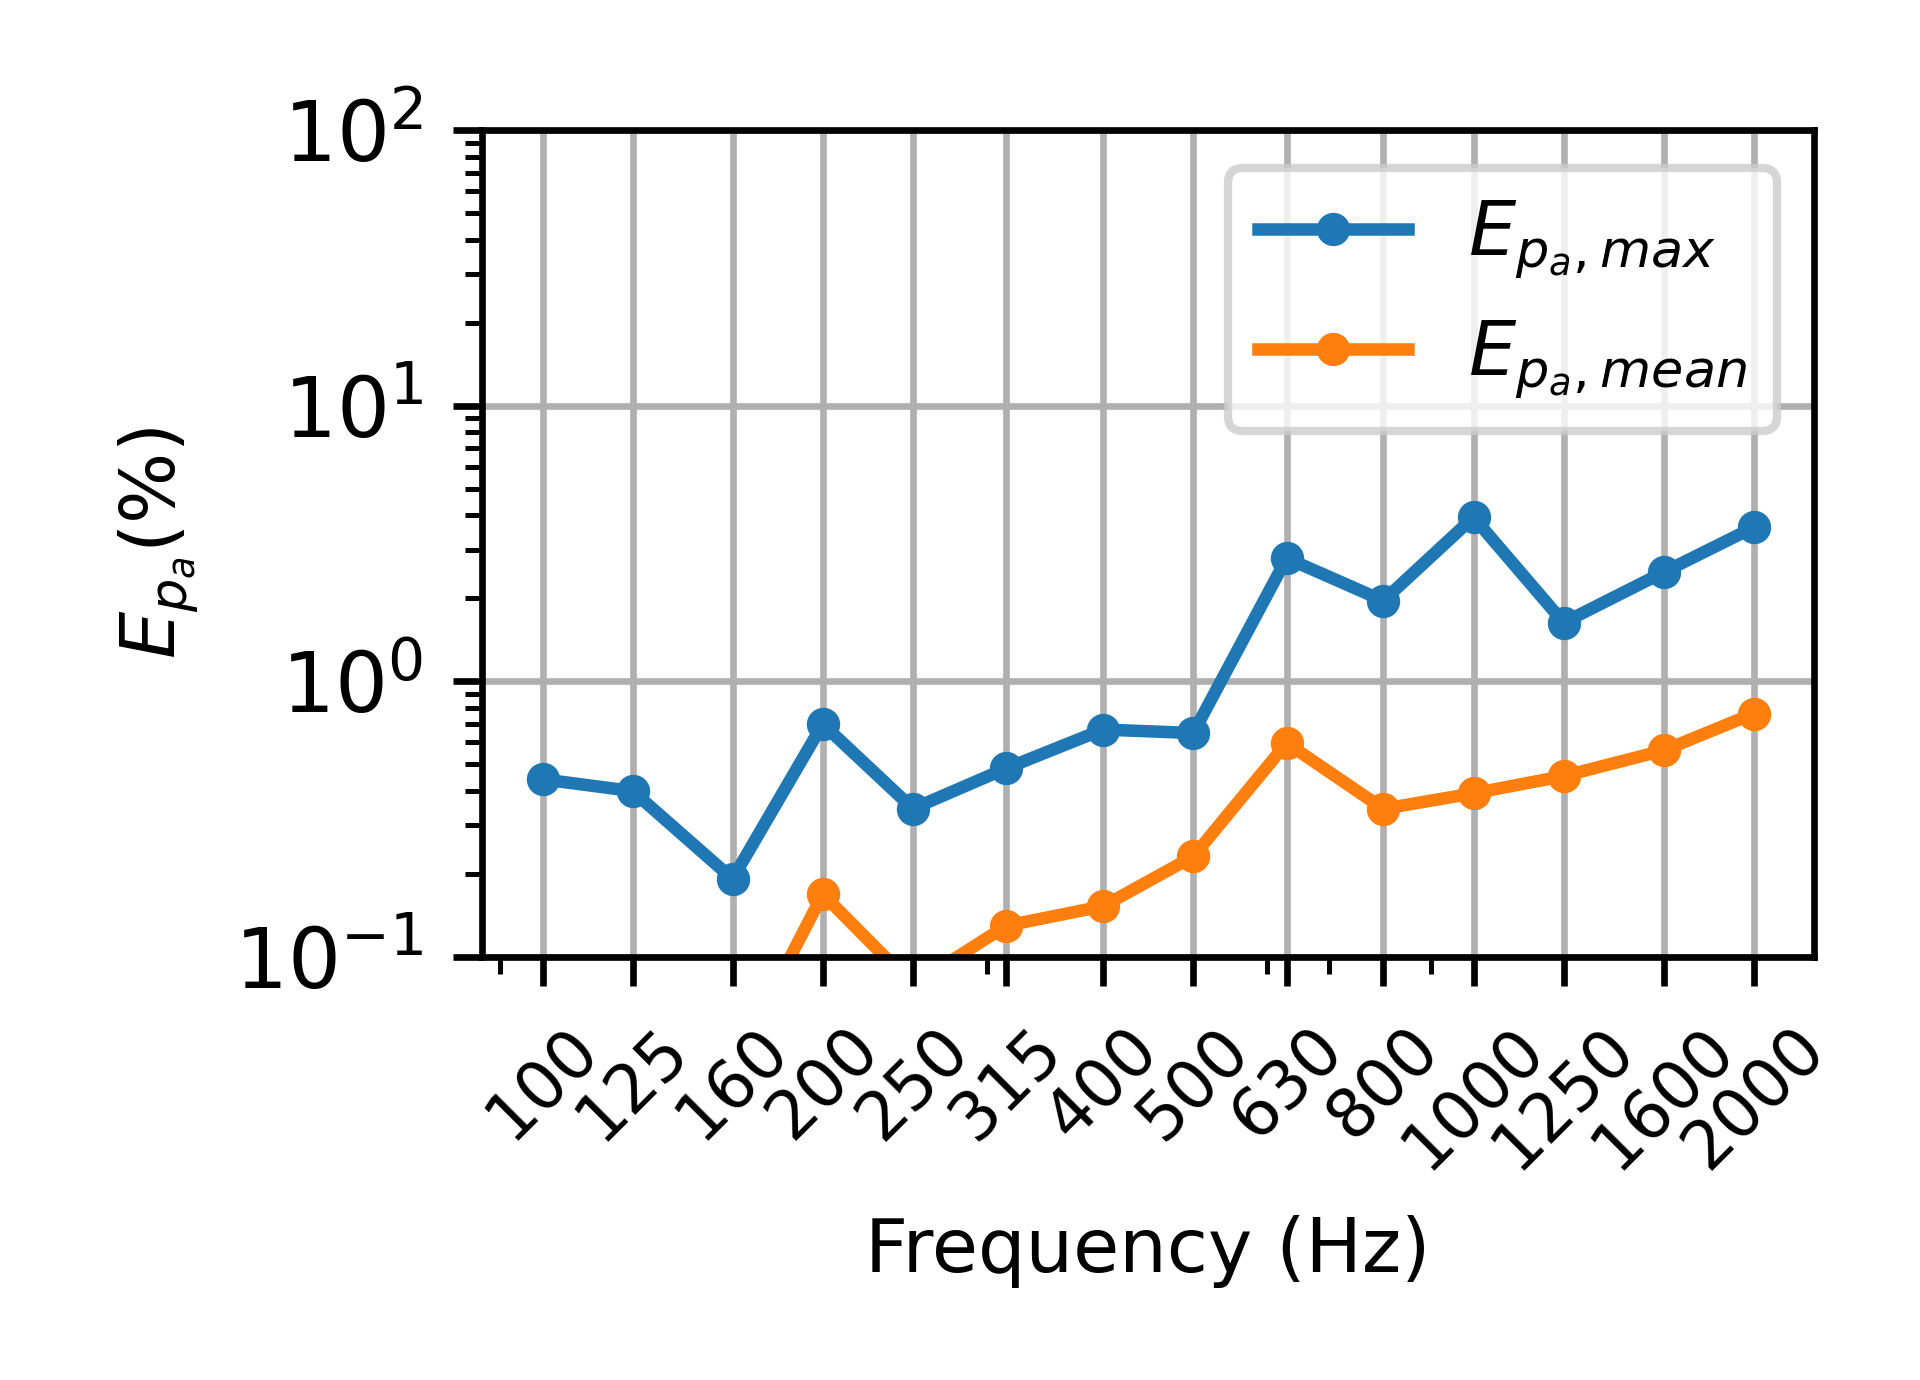
\includegraphics{fig/chap4/simulation_domain/width_1pt5m.png}
		\caption{\SI{1.5}{\meter}}
	\end{subfigure}
	\caption{The maximum relative error $E_{p_a,\text{max}}$ and the mean relative error $E_{p_a,\text{mean}}$ of one-third octave center frequencies for different domain widths.}
	\label{fig:relative_error_spectrum}
\end{figure}

\begin{table}
	\centering
	\caption{Computed errors (in \%) in the acoustic pressure for different domain widths.}
	\label{tab:computed_errors}
	\begin{tabular}{crrrrrrrr}
		\toprule
		 & \multicolumn{2}{c}{\SI{0.2}{\meter}} & \multicolumn{2}{c}{\SI{0.5}{\meter}} & \multicolumn{2}{c}{\SI{1}{\meter}} & \multicolumn{2}{c}{\SI{1.5}{\meter}} \\ \cmidrule(lr){2-3} \cmidrule(lr){4-5} \cmidrule(lr){6-7} \cmidrule(lr){8-9}
		 Frequency (Hz)& $E_{p_a,\text{max}}$  & $E_{p_a,\text{mean}}$ & $E_{p_a,\text{max}}$ & $E_{p_a,\text{mean}}$ & $E_{p_a,\text{max}}$ & $E_{p_a,\text{mean}}$ & $E_{p_a,\text{max}}$ & $E_{p_a,\text{mean}}$ \\
		 \midrule
		 100 & 22.40 & 4.67 & 7.72 & 1.54 & 1.77 & 0.33 & 0.44 & 0.08 \\ 
		 125 & 17.36 & 3.81 & 6.02 & 1.36 & 1.49 & 0.32 & 0.40 & 0.08 \\ 
		 160 & 20.35 & 5.17 & 5.21 & 1.02 & 0.76 & 0.13 & 0.19 & 0.04 \\ 
		 200 & 33.01 & 11.89 & 11.73 & 3.42 & 2.45 & 0.57 & 0.70 & 0.17 \\ 
		 250 & 45.14 & 13.32 & 11.40 & 2.59 & 1.36 & 0.25 & 0.34 & 0.08 \\ 
		 315 & 28.48 & 9.11 & 8.91 & 2.20 & 1.44 & 0.30 & 0.48 & 0.13 \\ 
		 400 & 20.19 & 5.87 & 5.38 & 1.93 & 1.85 & 0.45 & 0.67 & 0.15 \\ 
		 500 & 38.88 & 13.65 & 12.67 & 3.51 & 2.55 & 0.54 & 0.65 & 0.23 \\ 
		 630 & 58.67 & 17.33 & 20.67 & 6.31 & 4.77 & 1.38 & 2.80 & 0.60 \\ 
		 800 & 36.81 & 11.71 & 9.89 & 2.46 & 1.39 & 0.28 & 1.96 & 0.34 \\ 
		 1000 & 34.36 & 10.98 & 9.63 & 2.36 & 1.47 & 0.33 & 3.94 & 0.39 \\ 
		 1250 & 36.77 & 10.86 & 9.79 & 2.18 & 2.70 & 0.91 & 1.63 & 0.45 \\ 
		 1600 & 21.59 & 6.71 & 25.76 & 4.85 & 9.34 & 1.50 & 2.49 & 0.56 \\ 
		 2000 & 67.73 & 22.74 & 25.95 & 8.66 & 4.67 & 1.26 & 3.62 & 0.76 \\
		 \bottomrule		
	\end{tabular}
\end{table}


\newpage
\subsection*{Computational effort of the finite element model}

During the domain width parameter study, the computational effort of the finite element model used for the acoustic simulation of the X-Wagen was also evaluated. In the final model setup, a domain width of \SI{1.5}{\meter} is applied to the computational grid for frequency bands \SIrange{100}{800}{\hertz}, while the other grids for higher frequency bands have a domain width of \SI{1}{\meter}. In the simulation setup, each frequency band is resolved by 9 intermediate frequencies i.e. 9 harmonic steps have to be computed per analyzed one-third octave band. In this thesis, all computations were performed on the Sessanta server of the Institute of Mechanics and Mechatronics of TU Wien, which is equipped with 1 Terabyte RAM and two AMD EPYC 7542 32-core processors. The simulations were run with openCFS using 32 physical cores and the obtained computational efforts of the final design of the finite element model are listed in \cref{tab:computational_effort}. As can be read from the results, the computational effort of the model consisting of the required memory the computation time increase with the total unknowns i.e. nodes in the computational grid. While the computation time for the coarsest grid is only half an hour, the highest frequency band needs almost 24-fold the time to compute. The total computation time of the model is calculated as $10\times 0.5\,\text{h} + 2\times 2\,\text{h} + 5.5\,\text{h} + 12\,\text{h} = 24.5\,\text{h}$. One can see that almost half of the total computation time was spent on the computation of the highest frequency band. The total computation time was obtained by running the simulation jobs in a sequential order, the actual computation time can be shorten if the jobs are executed in a parallel manner. If the computation time is not considered, the upper limit of the frequency band that can be analyzed is restricted by the required memory, since this is rising with the degrees of freedom in the computational mesh. In a three-dimensional acoustic problem, a doubling of the analyzed frequency while keeping the same discretization size would leads to a 8 times larger degrees of freedom in the system, since the number of elements is also doubled in each spatial direction. That means, with a given amount of the memory, the size of the acoustic domain needs to be more confined if a analysis using higher frequency bands is of interest. For our finite element model, the required memory for the highest frequency band is about \SI{260}{\giga\byte}, without making the acoustic domain much smaller, it is not possible to increase the frequency range of interest.

\begin{table}[H]
	\centering
	\caption{Computational effort of the final model.}
	\label{tab:computational_effort}
	\begin{tabular}{ccccc}
		\toprule
		& Domain width & Total unknowns & Required RAM & Solve time (9 harmonic steps) \\
		\midrule
		Grid 1 & \SI{1.5}{\meter} & 0.8 Million & 20 GB & 0.5 hours \\
		Grid 2 & \SI{1}{\meter} & 2.3 Million & 70 GB & 2 hours \\
		Grid 3 & \SI{1}{\meter} & 4.4 Million & 150 GB & 5.5 hours \\
		Grid 4 & \SI{1}{\meter} & 6.6 Million & 260 GB & 12 hours \\
		\bottomrule
	\end{tabular}
\end{table}



\newpage
\section{Boundary conditions and loads}
\label{section:boundary_conditions}

\begin{figure}
	\centering
	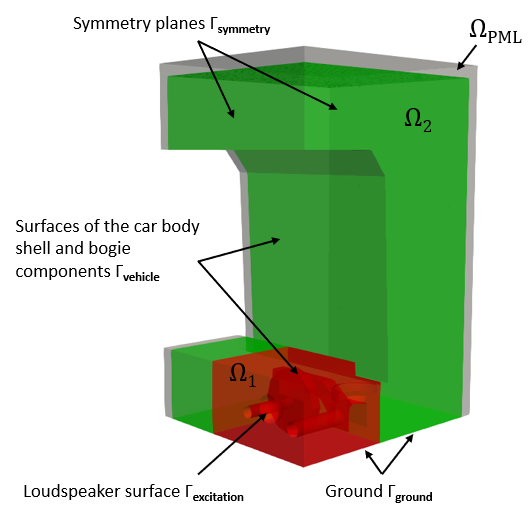
\includegraphics{fig/chap4/region_labels.png}
	\caption{Boundary surfaces of the finite element model.}
	\label{fig:boundary_conditions}
\end{figure}

After the considerations of the geometrical model in the previous section, the physical modeling aspects will be now discussed. In the finite element model of the X-Wagen, two boundary conditions of Neumann type are used, which are the sound hard boundary condition and the normal velocity boundary condition, respectively. The boundary surfaces of the model are shown in \cref{fig:boundary_conditions}. The concrete ground $\Gamma_{\text{ground}}$ and the wrapped surfaces of the car body shell and the bogie components $\Gamma_{\text{vehicle}}$ are assumed to be fully reflective. This also applies to the both symmetry planes (X-Y and Z-Y plane) of the quarter model $\Gamma_{\text{symmetry}}$. Hence, the sound hard boundary condition is used for these surfaces
\begin{equation}
	\nabla p_a \cdot \boldsymbol{n} = 0\qquad\text{on}\qquad\Gamma_{\text{ground}}\,\cup\,\Gamma_{\text{vehicle}}\,\cup\,\Gamma_{\text{symmetry}}\,.
\end{equation}
The acoustic excitation of the computational model comes from the loudspeaker, at which a normal velocity boundary condition is defined on its surface $\Gamma_{\text{excitation}}$, which reads as
\begin{equation}
	\boldsymbol{u_a} \cdot \boldsymbol{n} = u_{n}\qquad\text{on}\qquad\Gamma_{\text{excitation}}\,.
\end{equation}
However, the sound source characterization measurement from \cref{section:SWL_measurement} results in a acoustic power spectrum, which can not be directly applied to the finite element model. Therefore, a modeling approach of the sound source has to be found that can relate the surface normal velocity with the acoustic power.

\subsection*{Modeling of the sound source}

In the following, the modeling approach of the sound source is explained. Thereby, the loudspeaker sound source is modeled as a pulsating sphere radiating into free field, which is excited by a prescribed surface normal velocity with amplitude $\hat{u}_s = \hat{u}_a(a)$ with $a$ being the radius of the sphere. The pressure amplitude of the spherical wave at a distance $r$ from the sound source is given by
\begin{equation}
	\hat{p}_a(r) = \frac{\hat{A}}{r}\,e^{-jkr}\,, \label{eq:sound_pressure}
\end{equation}
with $\hat{A}$ being the monopole amplitude and $k$ being the wave number of the propagating wave. The relationship between the pressure amplitude and the amplitude of the particle velocity is described by the specific acoustic impedance, which for spherical wave computes by
\begin{equation}
	Z(r) = \frac{\hat{p}_a(r)}{\hat{u}_a(r)} = \rho_0 c_0\frac{jkr}{1+jkr}\,, \label{eq:specific_impedance}
\end{equation}
where $\rho_0$ is the density of the propagation medium and $c_0$ is the speed of sound in the medium. The product $Z_0 = \rho_0 c_0$ is also called the characteristic impedance of the propagation medium. The particle velocity of the spherical wave can then be expressed by
\begin{equation}
	\hat{u}_a(r) = \frac{\hat{p}_a(r)}{Z(r)} = \frac{\hat{A}}{r Z_0}\,e^{-jkr}\left(1+\frac{1}{jkr}\right)\,. \label{eq:sound_velocity}
\end{equation}
For stationary sound field, the average power density or the sound intensity is given by
\begin{equation}
	I(r) = \frac{1}{2}\text{Re}\lbrace\hat{p}_a(r)\hat{u}_a^*(r)\rbrace\,, \label{eq:sound_intensity}
\end{equation}
where $()^*$ denotes the complex conjugate. By inserting \cref{eq:sound_pressure} and \cref{eq:sound_velocity} into the expression of the sound intensity, one obtains
\begin{align}
	I(r) &= \frac{1}{2}\text{Re}\lbrace \frac{\hat{A}\hat{A}^*}{r^2 Z_0}\,e^{-jkr}\,e^{jkr}\left(1+j\frac{1}{kr}\right)\rbrace \\
		 &=\frac{1}{2}\frac{|\hat{A}|^2}{r^2Z_0}\,.
\end{align}
Furthermore, the acoustic power $W$ of a steady sound source radiating into free field is obtained by integrating the sound intensity $I(r)$ over a surface $\Gamma$ enclosing the sound source and can be found as
\begin{align}
	W &= \oint_{\Gamma} I(r) \dif\Gamma \\
	  &= \bar{I}(r)\,4\pi r^2 \\
	  &= \frac{2\pi |\hat{A}|^2}{Z_0}\,. \label{eq:acoustic_power}
\end{align}
As apparent in \cref{eq:acoustic_power}, the acoustic power is independent from the distance to the sound source and can be related to the monopole amplitude $\hat{A}$. Assume a sound source has a radius of $a$, the pressure amplitude on the sound source surface $\hat{p}_s = \hat{p}_a(a)$ can be expressed by the product of the surface normal velocity $\hat{u}_s = \hat{u}_a(a)$ and the specific impedance $Z(a)$ evaluated at the source surface and is found by
\begin{equation}
	\hat{p}_s = \hat{p}(a) = \hat{u}_s Z(a) = \frac{\hat{A}}{a}\,e^{-jka}\,.
\end{equation}
Upon bringing the monopole amplitude $\hat{A}$ to one side of the equation, and evaluating \cref{eq:specific_impedance} at the source radius $a$, one obtains
\begin{align}
	\hat{A} &= a\hat{u}_s Z(a)\,e^{jka} \\
			&= a\hat{u}_s Z_0 \frac{jka}{1+jka}\,e^{jka}\,. \label{eq:monopole_amplitude}
\end{align}
By inserting \cref{eq:monopole_amplitude} into \cref{eq:acoustic_power}, the acoustic power $W$ can hence be expressed by the surface normal velocity $\hat{u}_s$, which reads as
\begin{equation}
	W = 2\pi a^2 Z_0 \left|\hat{u}_s\right|^2\frac{(ka)^2}{1+(ka)^2} \,.
\end{equation}
Assuming that the surface normal velocity contains only real part i.e. $\left|\hat{u}_s\right| = \hat{u}_s$, one obtains
\begin{equation}
	\hat{u}_s = \sqrt{\frac{W(1 + k^2a^2)}{2\pi Z_0 k^2a^4}}\,. \label{eq:input_velocity}
\end{equation}
Through \cref{eq:input_velocity}, the required normal velocity at the loudspeaker surface $\Gamma_{\text{excitation}}$ for a given acoustic power can be calculated. Therefore, the measured acoustic power spectrum of the sound source (see \cref{fig:average_SWL}) can be converted into a surface normal velocity spectrum, which is shown in \cref{fig:input_SVL}.

\begin{figure}
	\centering
	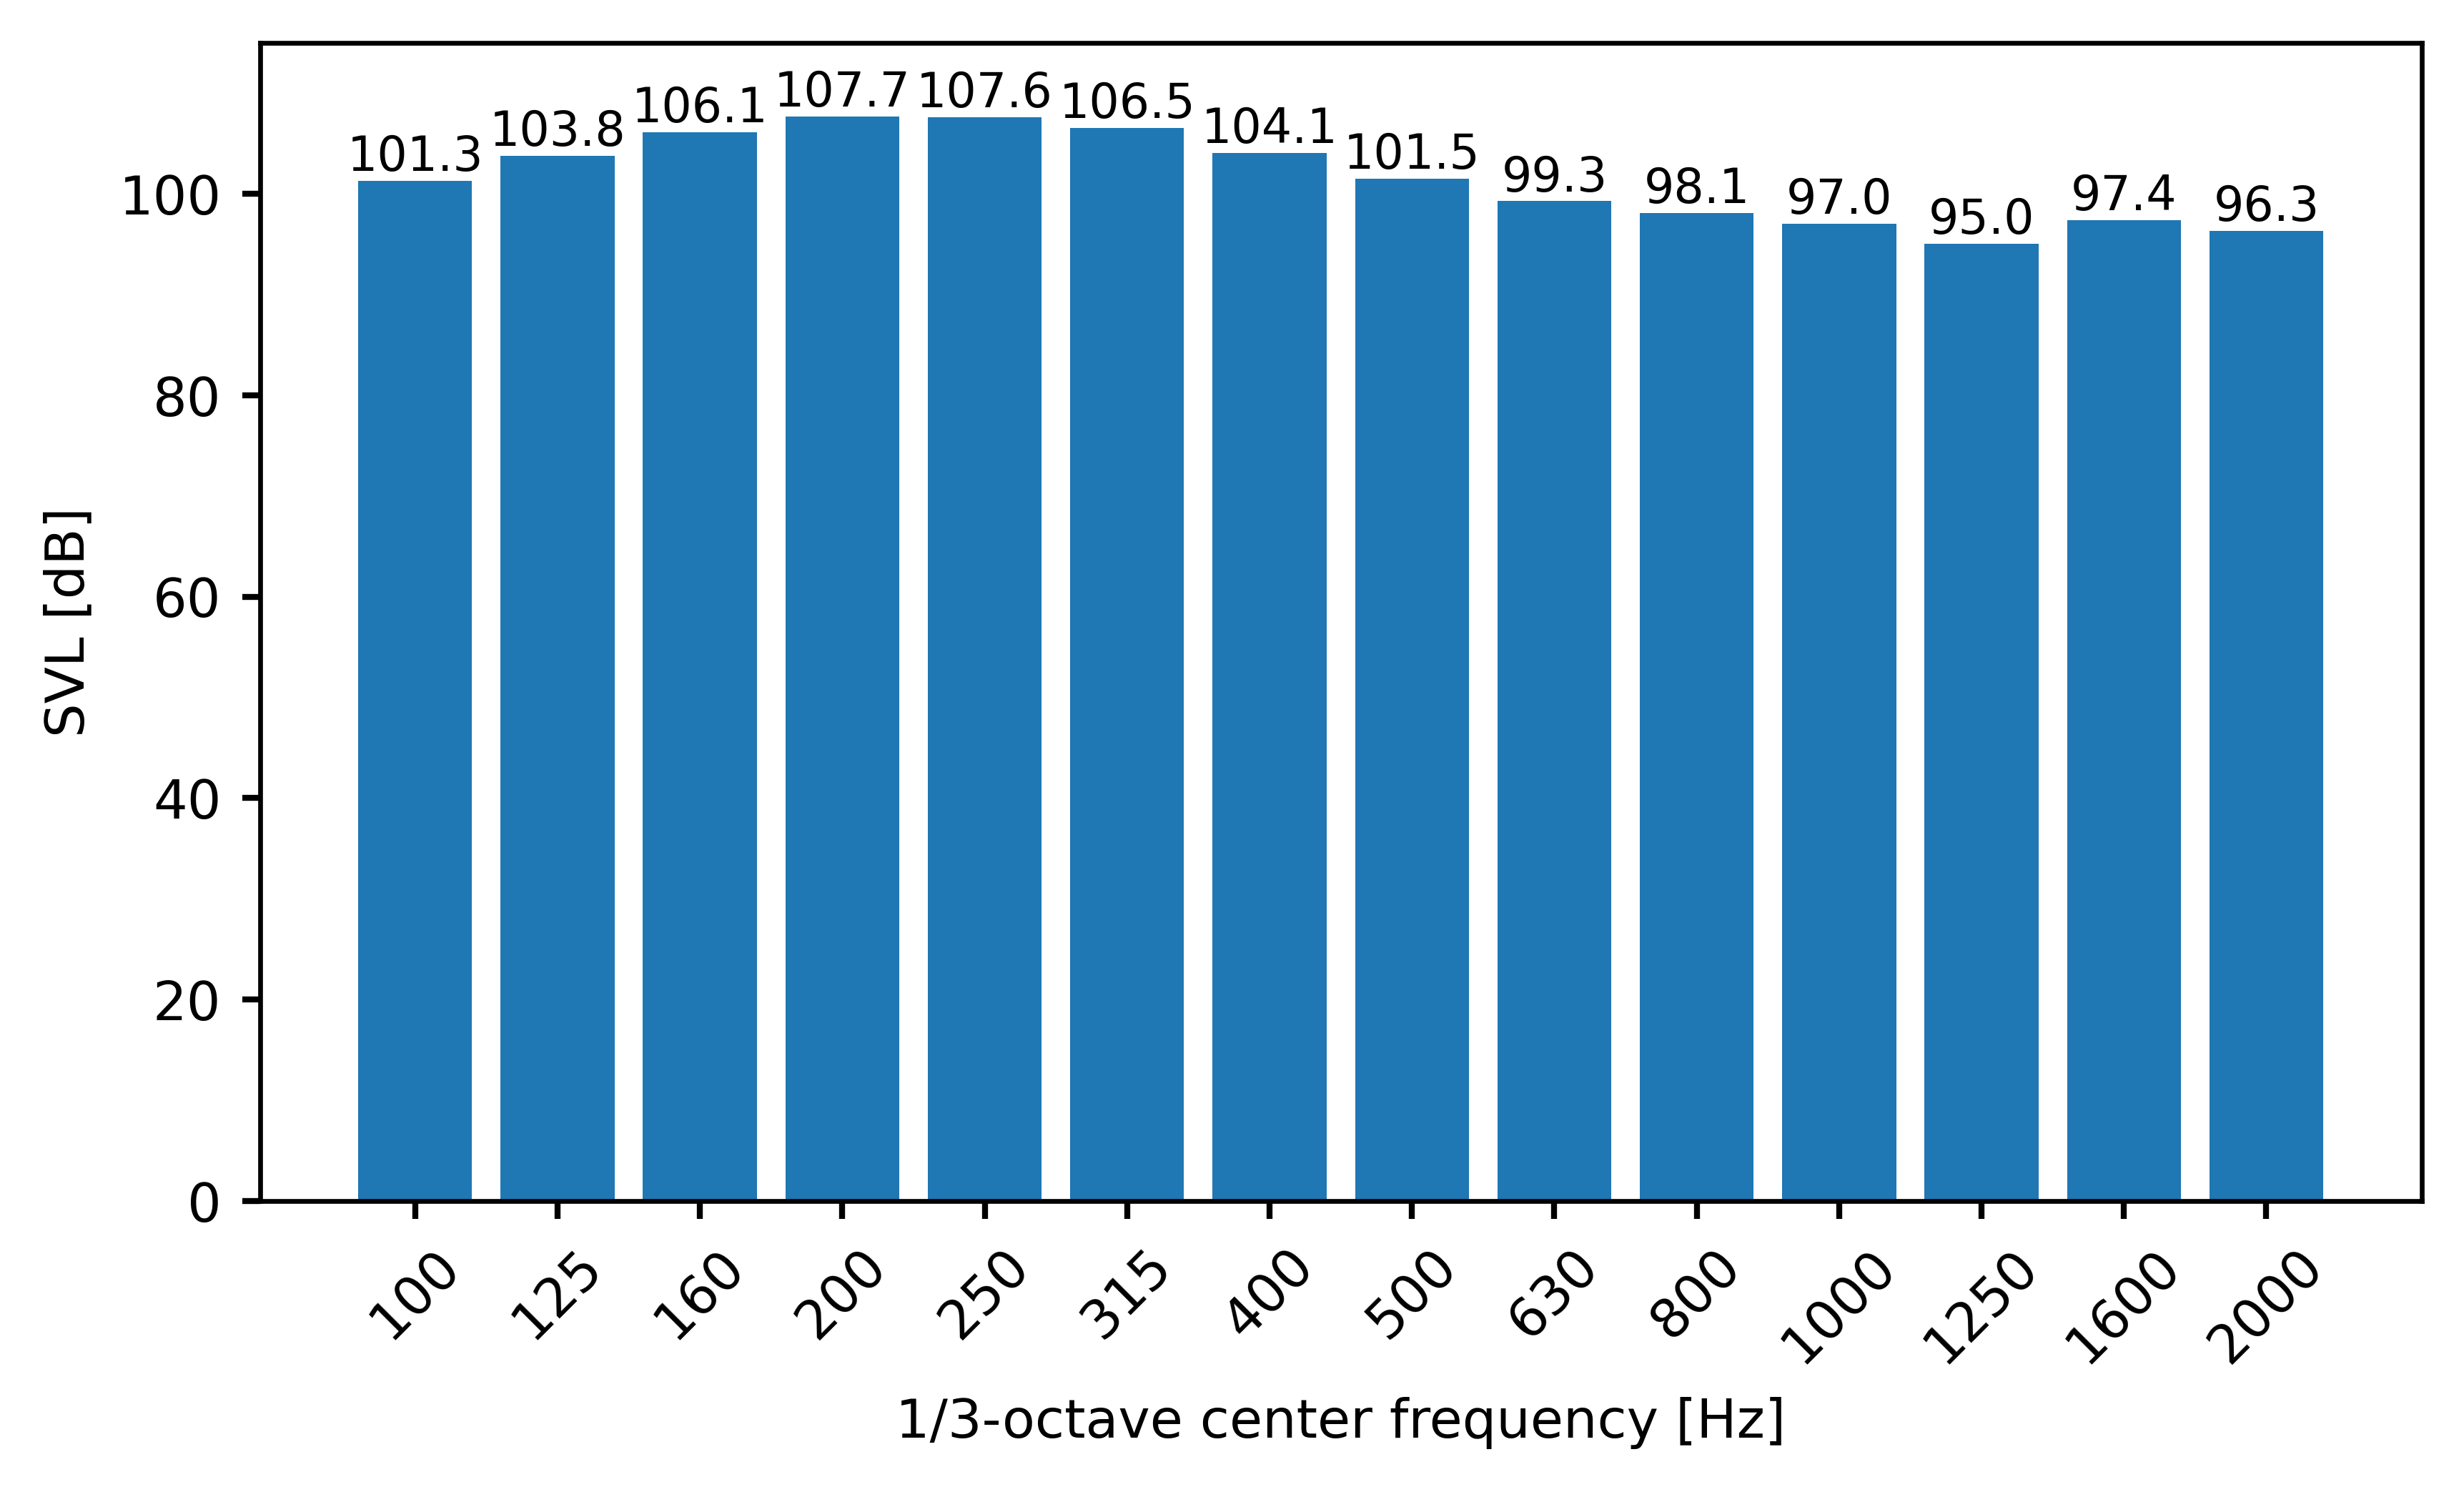
\includegraphics{fig/chap4/input_SVL.png}
	\caption{SVL spectrum of the surface normal velocity in dB ref. $5\cdot10^{-8}\,\text{m/s}$, calculated from the measured acoustic power spectrum (\cref{fig:average_SWL}) using \cref{eq:input_velocity}.}
	\label{fig:input_SVL}
\end{figure}

%\section{General simulation setup}
\newpage
\section{Parametric study}
\label{section:parametric_study}
\subsection{Variation of underfloor geometry}
\label{section:variation_geometry}

In the initial geometric setup, the contemplated underfloor components in the finite element model are the bogie frame, the wheel with axle, and the air suspension. In order to investigate the stability of simulation results to different underfloor geometrical setups, a parametric study with a variation of the underfloor geometry is carried out in the following.

\begin{figure}[H]
	\centering
	\begin{subfigure}[b]{0.49\textwidth}
		\centering
		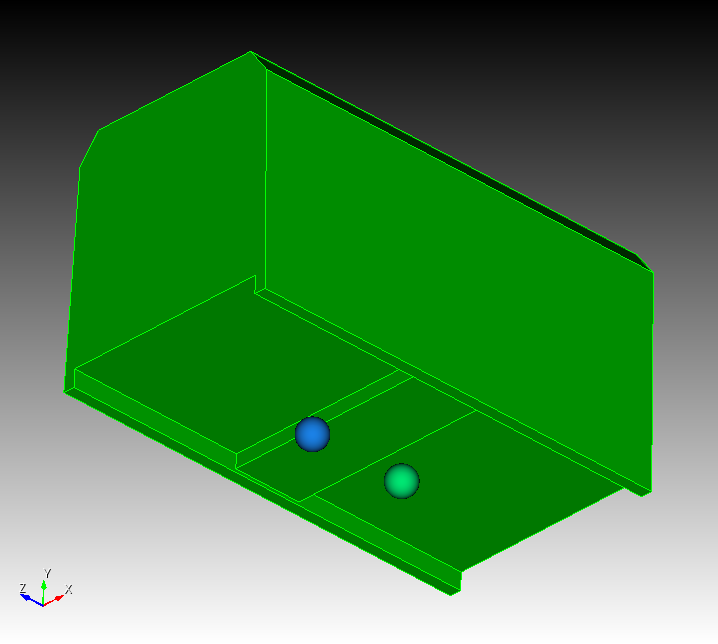
\includegraphics[width = 0.8\linewidth]{fig/chap4/geometry/no_underfloor_components_2.png}
		\caption{No underfloor components}
		\label{fig:no_underfloor_components}
	\end{subfigure}
	\begin{subfigure}[b]{0.49\textwidth}
		\centering
		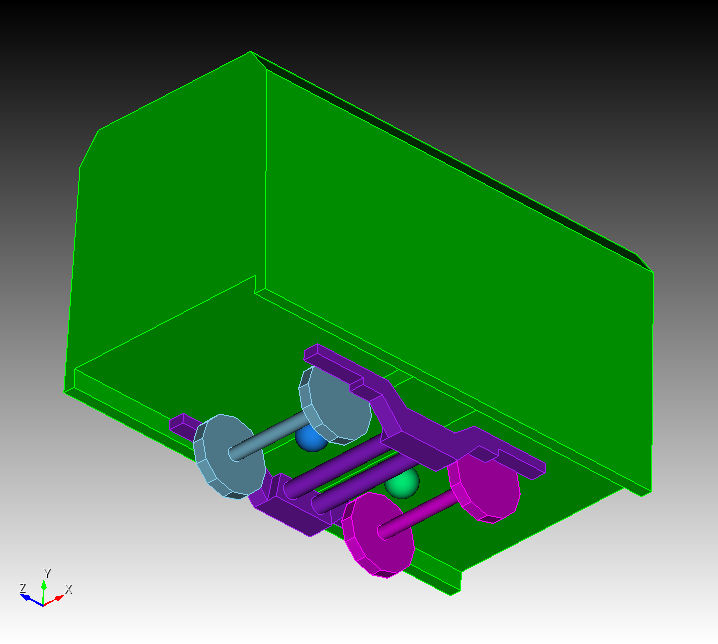
\includegraphics[width = 0.8\linewidth]{fig/chap4/geometry/no_air_suspension_2.png}
		\caption{No air suspension}
		\label{fig:no_air_suspension}
	\end{subfigure}
	\begin{subfigure}[b]{0.49\textwidth}
		\centering
		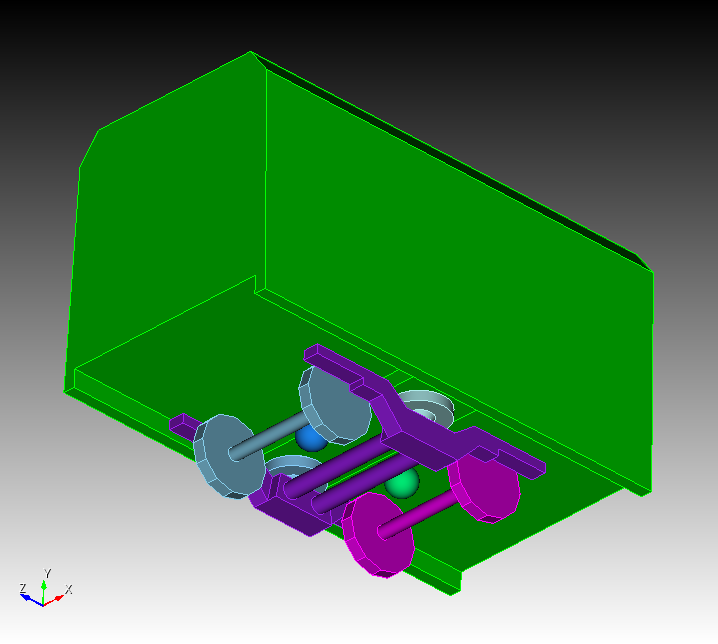
\includegraphics[width = 0.8\linewidth]{fig/chap4/geometry/initial_model_2.png}
		\caption{Initial model}
		\label{fig:initial_model}
	\end{subfigure}
	\begin{subfigure}[b]{0.49\textwidth}
		\centering
		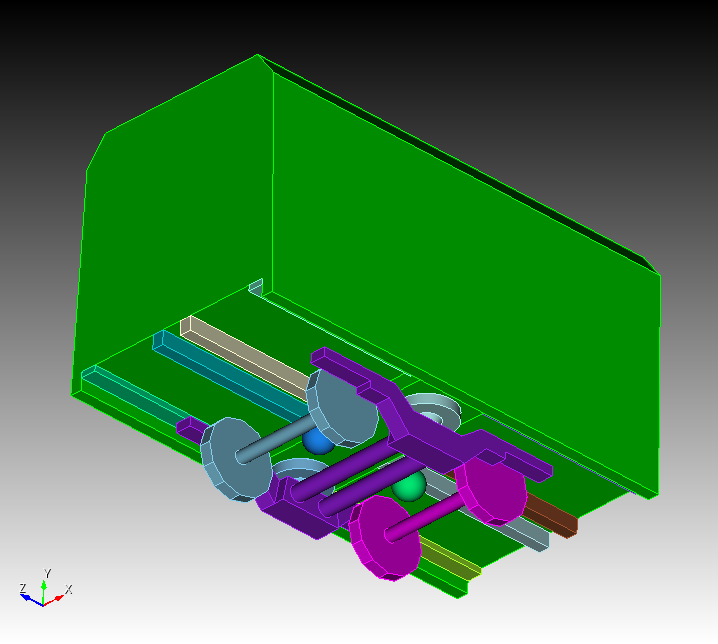
\includegraphics[width = 0.8\linewidth]{fig/chap4/geometry/additional_structures.png}
		\caption{Additional structures}
		\label{fig:additional_structures}
	\end{subfigure}
	\caption{Underfloor geometry with four variations.}
	\label{fig:variation_underfloor}
\end{figure}

For the parametric study, four different variations of underfloor geometry including the initial finite element model as described in \cref{section:geometry} are prepared, which are shown in \cref{fig:variation_underfloor}, ordered by their complexity. Again, the full model of each geometry is shown for a better illustration, whereby the one-fourth model will be used for the simulation. The simplest model (\cref{fig:no_underfloor_components}) contains only the car body shell without any underfloor components, the blue or the green sphere beneath the car floor represents the omnidirectional loudspeaker. In the next more complex model (\cref{fig:no_air_suspension}), the bogie frame and the wheels are contemplated, and differs from the initial geometry (\cref{fig:initial_model}) only by the air suspension, that is why this variation is also named "no air suspension". Finally, the last geometrical model (\cref{fig:additional_structures}) is set up by attaching additional structures to the car floor, which represent the cable ducts beneath the car floor.

\newpage
\subsection{Variation of ground surface impedance}

In the initial simulation setup, the ground is modeled as a fully reflective surface at which the homogeneous Neunmann (sound hard) boundary condition is applied.
However, it would also be of interest to investigate the influence of including ground absorption on the simulation result.
An absorbing surface is characterized by its absorption coefficient $\alpha$, which is frequency dependent in most cases.
In the finite element formulation, the reflection and absorption of the incident acoustic wave at a surface is described by the surface impedance boundary condition, which can be related to the absorption coefficient of the surface. In the following, the relation between the absorption coefficient $\alpha$ and the surface impedance $Z_s$ is presented following Nedkov \cite{nedkov_impedance_2011}.

The sound absorption coefficient $\alpha$ of a material is defined by the ratio of the absorbed acoustic power $W_{\text{absorbed}}$ and the power of incident wave $W_{\text{incident}}$, which for wave at normal incidence reads as
\begin{equation}
	\alpha = \frac{W_{\text{absorbed}}}{W_\text{incident}} = 1 - |R|^2\,, \label{eq:absorption_coefficient}
\end{equation}
with $R$ being the complex reflection coefficient, which can be represented as
\begin{equation}
	R = \frac{Z_s - Z_0}{Z_s + Z_0} = \frac{\frac{Z_s}{Z_0} - 1}{\frac{Z_s}{Z_0} + 1}\,, \label{eq:reflection_coefficient}
\end{equation}
where $Z_0 = \rho_0 c_0$ is the characteristic impedance of the propagation medium and $Z_s$ is the specific acoustic impedance of the absorbing surface.
The impedance ratio $\frac{Z_s}{Z_0}$ is also called the normalized surface impedance
\begin{equation}
	\tilde{Z_s} = \frac{Z_s}{Z_0} = \tilde{R_s} + j\tilde{X_s}\,,
\end{equation}
which can be slit into a real part $\tilde{R_s}$ and an imaginary part $\tilde{X_s}$. By inserting \cref{eq:reflection_coefficient} into \cref{eq:absorption_coefficient}, the absorption coefficient $\alpha$ can be related to the complex surface impedance by
\begin{equation}
	\alpha = \frac{4\tilde{R_s}}{\tilde{R_s}^2+\tilde{X_s}^2 + 2\tilde{R_s} + 1} \,. \label{eq:absorption_coefficient_2}
\end{equation}
In order to uniquely define the surface impedance $\tilde{Z_s}$ of the absorbing surface for a given normal incident absorption coefficient $\alpha$, the phase of the complex surface impedance also has to be known, which is given by
\begin{equation}
	 \varphi = \arctan{\frac{\tilde{X_s}}{\tilde{R_s}}}\,. \label{eq:impedance_phase_angle}
\end{equation}
The impedance characteristic of a ground surface can be determined for example by an in-situ measurement using impedance tube method \cite{wolkesson_2013,Seybert2008MeasurementOP}.
For the case that a measurement is not accessible, the absorption data can be retrieved e.g. from a acoustic data bank, which, in most cases, provides only the absorption coefficient spectrum in stead of the complex surface impedance.
However, it has been shown that also the phase has to be provided to uniquely define the surface impedance for a given absorption coefficient.
In order to have an idea how the missing information of the impedance phase angle affects the simulation result, surface impedance boundary condition is prescribed at the ground of the finite element model using varying impedance phase angle.

\begin{figure}[H]
	\centering
	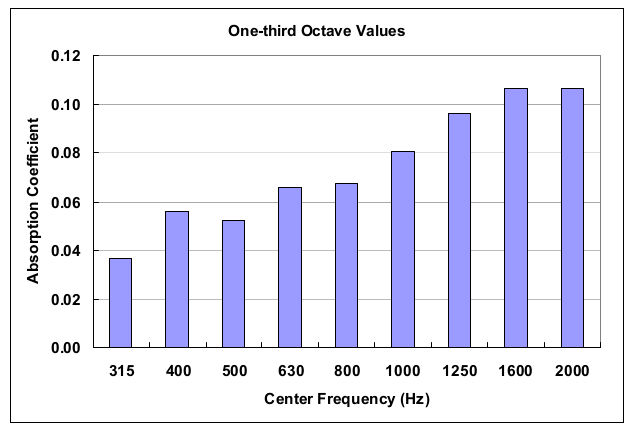
\includegraphics[width=0.7\textwidth]{fig/chap4/impedance/absorption_spectrum.png}
	\caption{Absorption coefficient in one-third octave bands \cite{Seybert2008MeasurementOP}}
	\label{fig:ground_absorption}
\end{figure}

Due to a missing ground absorption measurement, the absorption spectrum from the pavement absorption measurement carried out by Seybert et al. \cite{Seybert2008MeasurementOP} is used, which is shown in \cref{fig:ground_absorption}.
The values of the absorption coefficients are estimated from the graph and are listed in \cref{tab:absorption_coefficient} since these were not provided in the paper. For frequencies lower than \SI{315}{\hertz}, the absorption coefficient is set to 0.02. The complex normalized surface impedance can then be calculated by solving the system of equations consists of \cref{eq:absorption_coefficient_2} and \cref{eq:impedance_phase_angle}. Thereby, the impedance phase angle $\varphi$ is assumed to be \SI{0}{\degree} (only real part), $\pm$\SI{30}{\degree}, $\pm$\SI{45}{\degree}, and $\pm$\SI{60}{\degree}, respectively. The obtained normalized surface impedance spectra for different impedance phase angles are shown in \cref{fig:input_impedance}.

\begin{table}[H]
	\centering
	\caption{Estimated absorption coefficient from \cref{fig:ground_absorption}, for frequencies lower than 315 Hz the values are set to 0.02.}
	\label{tab:absorption_coefficient}
	\begin{tabular}{cccc}
		\toprule
		Frequency (Hz) & $\alpha$ & Frequency (Hz) & $\alpha$ \\
		\midrule
		100 & 0.02 & 500 & 0.05 \\
		125 & 0.02 & 630 & 0.065 \\
		160 & 0.02 & 800 & 0.065 \\
		200 & 0.02 & 1000 & 0.08 \\
		250 & 0.02 & 1250 & 0.095 \\
		315 & 0.035 & 1600 & 0.105 \\
		400 & 0.055 & 2000 & 0.105 \\
		\bottomrule
	\end{tabular}
\end{table}

\begin{figure}[H]
	\centering
	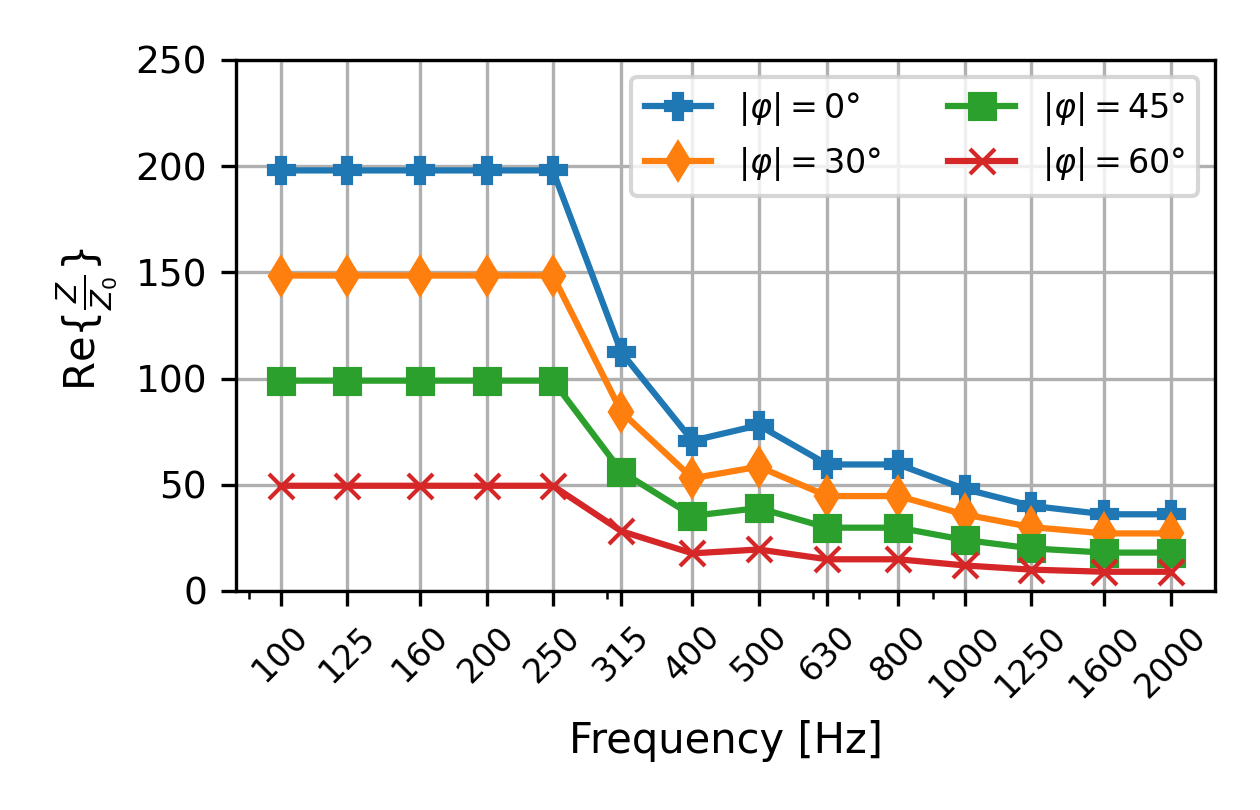
\includegraphics{fig/chap4/impedance/impedance_real.png}
	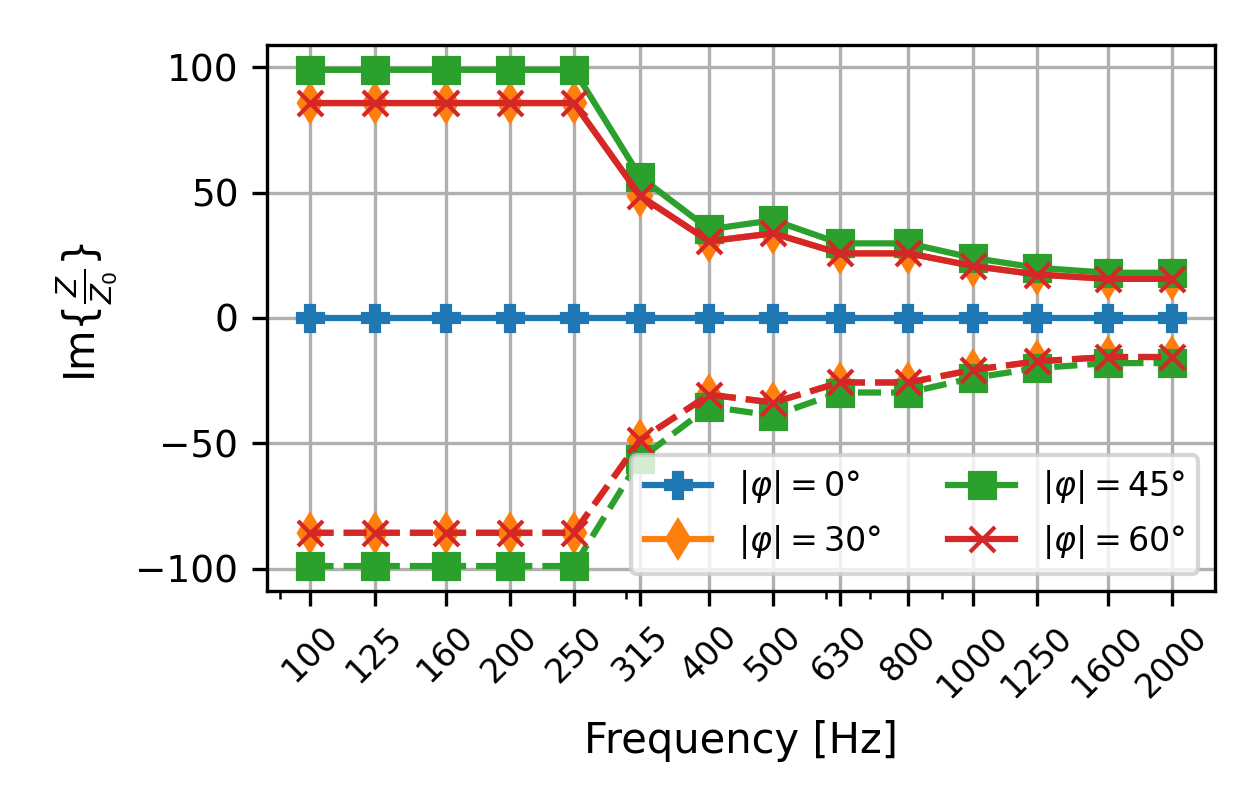
\includegraphics{fig/chap4/impedance/impedance_imag.png}
	\caption{Real and imaginary part of the surface impedance normalized by $Z_0 = \rho_0 c_0$ calculated by solving \cref{eq:absorption_coefficient_2} and \cref{eq:impedance_phase_angle}.}
	\label{fig:input_impedance}
\end{figure}

\newpage
\subsection{Variation of frequency steps per 1/3-octave band}

In this thesis, the simulation and the measurement results will be compared in one-third octave bands.
In the initial simulation setup, each one-third octave band is computed using nine intermediate frequency steps corresponding to the 1/24-octave center frequencies to ensure a sufficient frequency band resolution.
However, the computation time of single one-third octave band grows almost linearly with the number of intermediate frequency steps.
As already shown in \cref{section:geometry}, the computation time of the highest frequency band \SI{2000}{Hz} using nine intermediate frequencies almost takes up half of the total simulation run time.
Therefore, it would be of great interest to find a proper number of intermediate frequency steps per one-third octave band, which can lower the computational effort of the simulation while providing a similar numerical accuracy.

For the parametric study, each one-third octave band is computed using one, three, five, and nine intermediate frequency steps, respectively. Obviously, there are several possibilities for choosing the frequencies used within the octave band. However, this study concentrates on the influence of the number of frequencies used on the simulation results but not the different selection of the frequencies. Therefore, a rule for choosing the frequencies used within the one-third octave band will be defined for each number of steps. For the single frequency step, the center frequency of the corresponding one-third octave band is used. Next, for the model using three intermediate steps, the lower and the upper frequency limits of the one-third octave band are additionally used, corresponding to the 1/6-octave center frequencies. Finally, the frequencies used for five steps and nine steps are equivalent to the 1/12-octave center frequencies and the 1/24-octave center frequencies within the one-third octave frequency band, respectively. An example of the frequency selection for \SI{1000}{\hertz} one-third octave band is shown in \cref{tab:variation_freq_steps}. The same selection criteria apply to other one-third octave bands.

\begin{table}[H]
	\caption{Choice of frequencies used for different number of intermediate steps, example one-third octave band \SI{1000}{\hertz}.}
	\centering
	\begin{tabular}{ccc}
		\toprule
		Number of steps    &  Frequencies used (Hz) & Note  \\
		\midrule
		1    &  1000  & 1/3-octave center frequency\\
		3  	 &  891, 1000, 1122 & 1/6-octave center frequencies \\
		5  	 &  891, 944, 1000, 1059, 1122 & 1/12-octave center frequencies\\
		9    &  891, 917, 944, 972, 1000, 1029, 1059, 1091, 1122 & 1/24-octave center frequencies \\
		\bottomrule
	\end{tabular}
	\label{tab:variation_freq_steps}
\end{table}